\documentclass[a4paper, 11pt, oneside, polutonikogreek, english]{article}
\usepackage{lmodern}
\usepackage[T1]{fontenc}

% Load encoding definitions (after font package)

\usepackage{textalpha}

\usepackage[dvipsnames]{xcolor}
\usepackage{eso-pic,graphicx}
\usepackage[top=50mm, bottom=50mm, outer=29mm, inner=29mm]{geometry}
\setlength{\columnsep}{90pt}

\usepackage{listings}
\lstset{basicstyle=\ttfamily}

% Babel package:
\usepackage[english]{babel}

% With XeTeX$\$LuaTeX, load fontspec after babel to use Unicode
% fonts for Latin script and LGR for Greek:
\ifdefined\luatexversion \usepackage{fontspec}\fi
\ifdefined\XeTeXrevision \usepackage{fontspec}\fi

% ``Lipsiakos'' italic font `cbleipzig`:
\newcommand*{\lishape}{\fontencoding{LGR}\fontfamily{cmr}%
		       \fontshape{li}\selectfont}
\DeclareTextFontCommand{\textli}{\lishape}

\usepackage{booktabs}
\setlength{\emergencystretch}{15pt}

\usepackage{sectsty}
\usepackage[titles]{tocloft}

\sectionfont{\Huge}
\subsectionfont{\LARGE}
\subsubsectionfont{\Large}

\usepackage{setspace}
\onehalfspacing

\usepackage{float}
\usepackage{fancyhdr}
\usepackage{microtype}
% change color of text, example replace all \color{Goldenrod} with \color{lightgray}

\makeatletter % change only the display of \thepage, but not \thepage itself:
\patchcmd{\ps@plain}{\thepage}{\bfseries\large\color{SkyBlue}{\thepage}}{}{}
\makeatother

\color{SkyBlue}

\begin{document}
\bfseries
\pagestyle{plain} % after changing a pagestyle command, it's necessary to invoke it explicitly
\AddToShipoutPictureBG{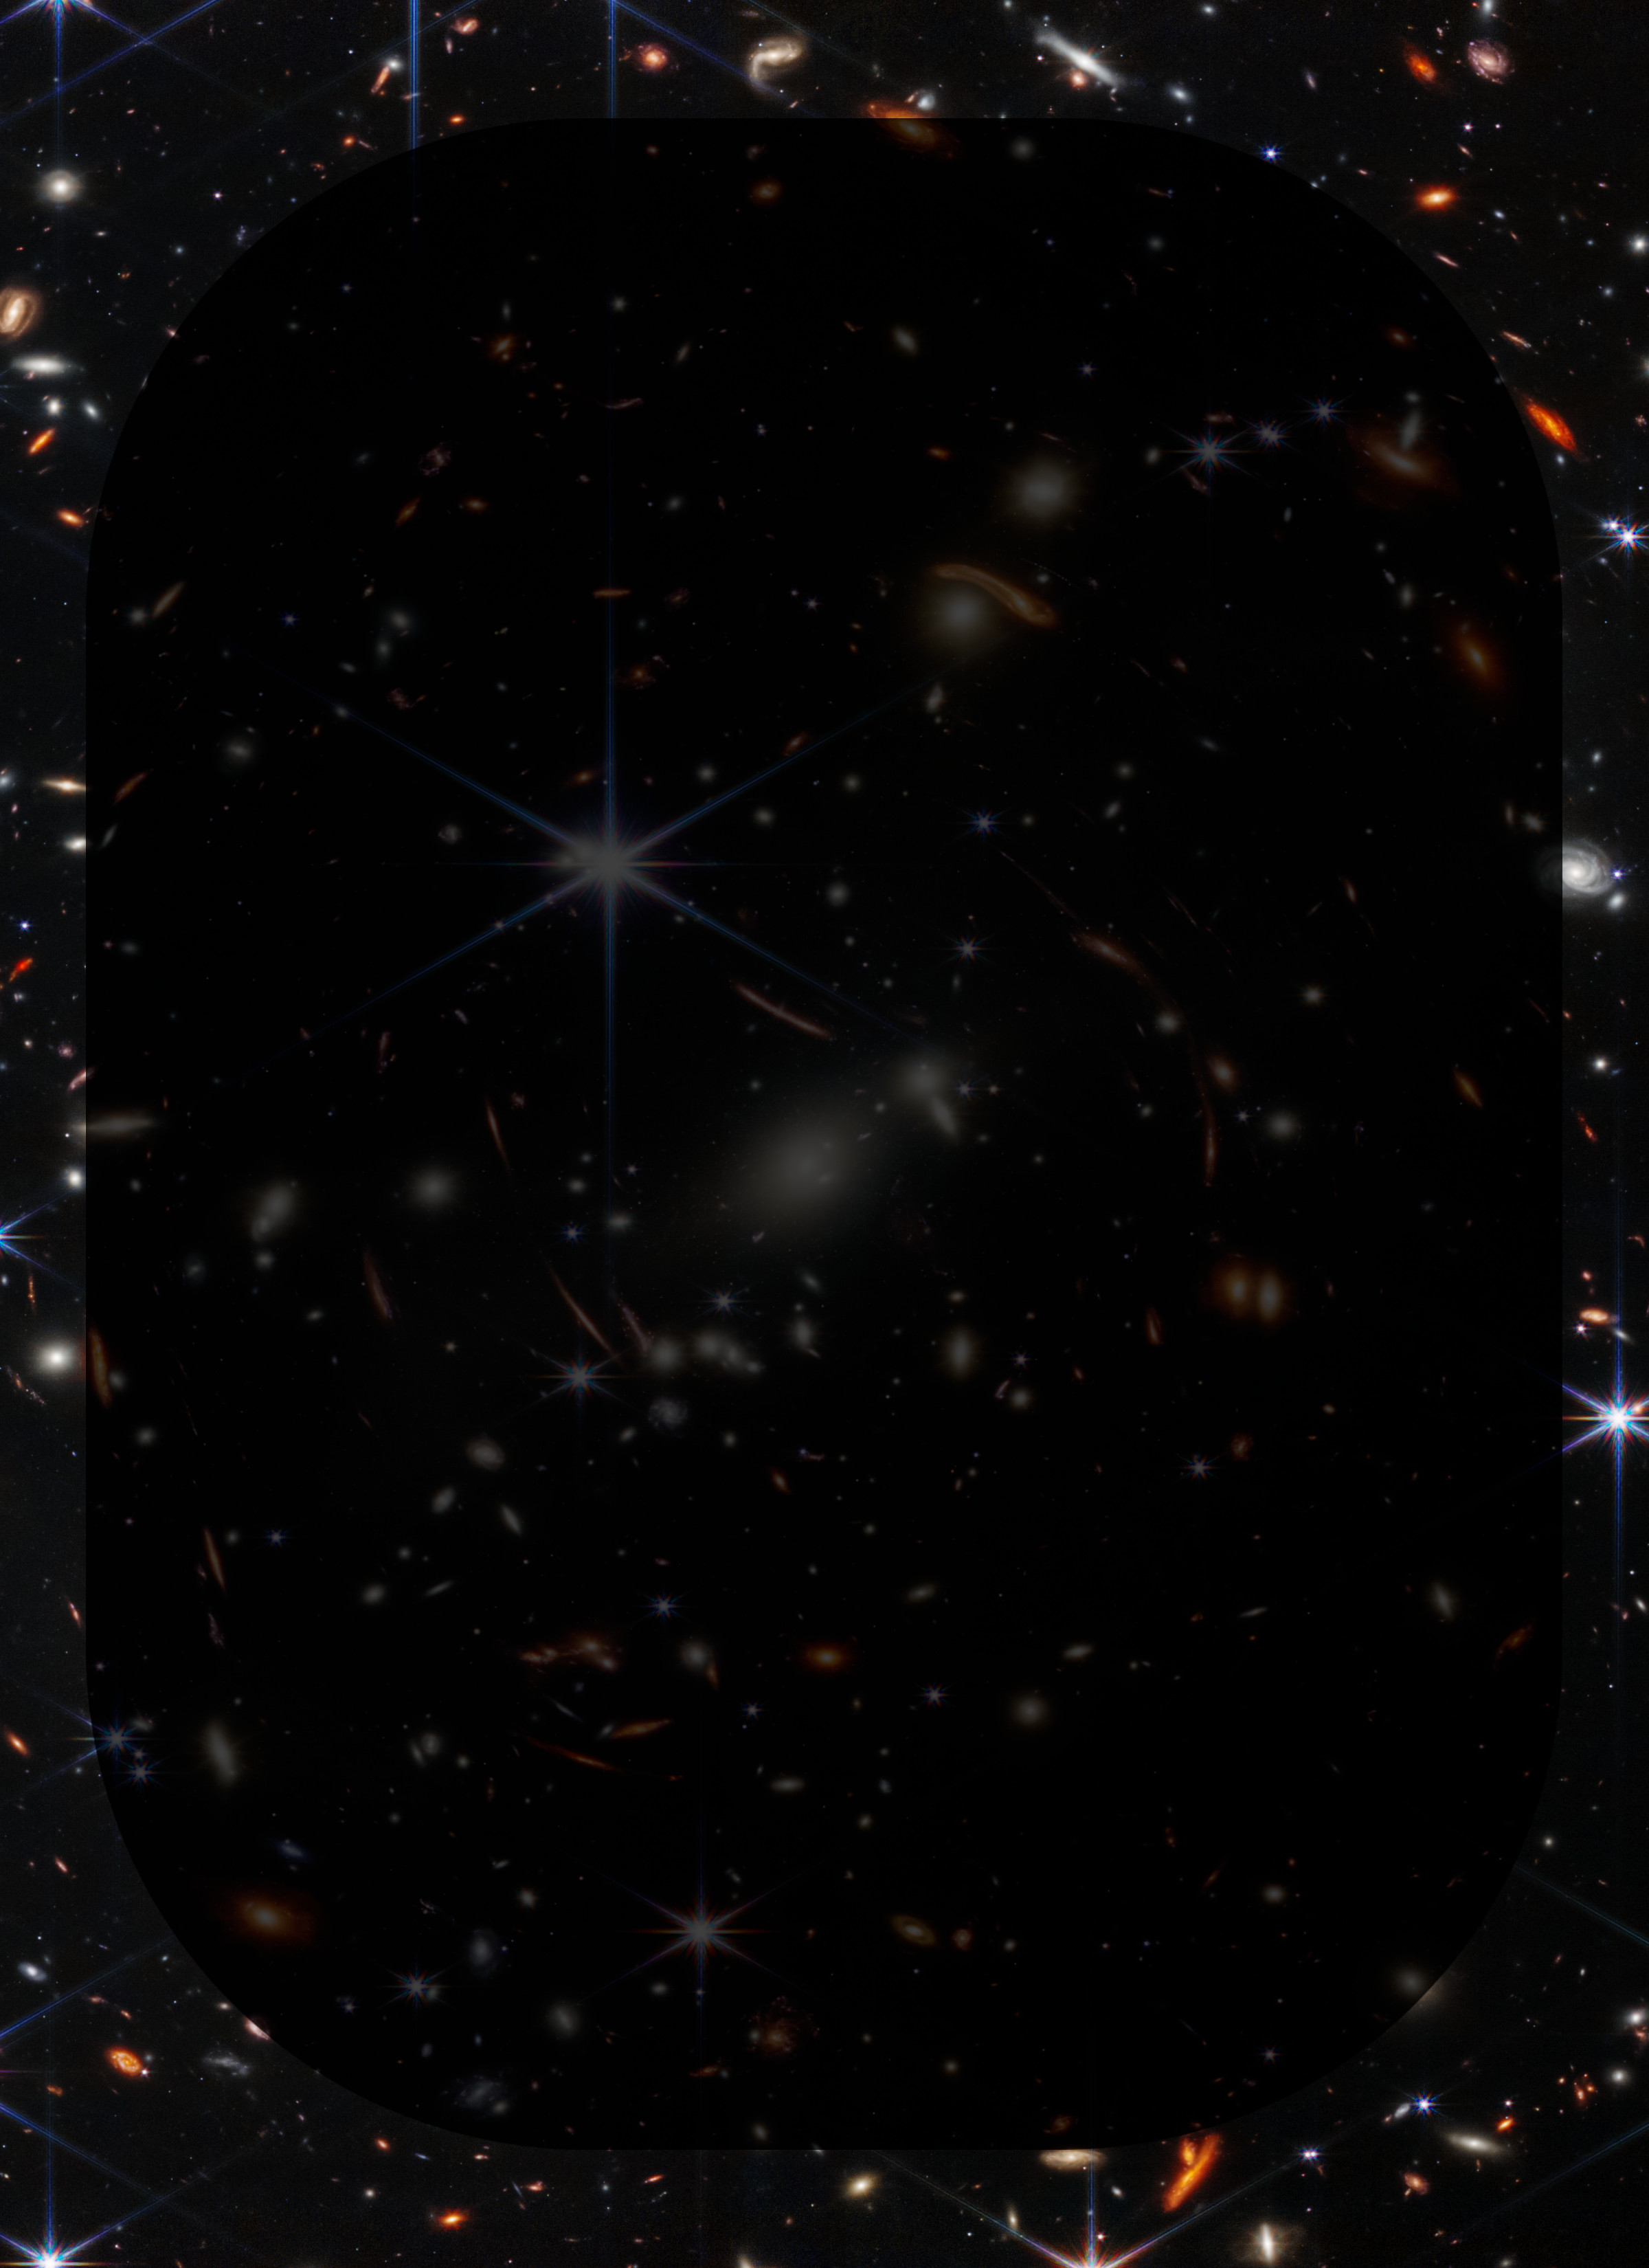
\includegraphics[width=\paperwidth,height=\paperheight]{webb-deepfield.jpeg}}

\renewcommand\thefootnote{{\bfseries\color{SkyBlue}{\arabic{footnote}}}}
\let\oldfootnote\footnote
    \renewcommand{\footnote}[1]{\oldfootnote{{\normalsize\bfseries\color{SkyBlue}#1}}}
\begin{titlepage} % Suppresses headers and footers on the title page
	\centering % Centre everything on the title page
	\scshape % Use small caps for all text on the title page

	%------------------------------------------------
	%	Title
	%------------------------------------------------
	
	\rule{\textwidth}{1.6pt}\vspace*{-\baselineskip}\vspace*{2pt} % Thick horizontal rule
	\rule{\textwidth}{0.4pt} % Thin horizontal rule
	
	\vspace{0.75\baselineskip} % Whitespace above the title

        {\LARGE The Probable Infinity \\of Nature and Life: \\Three Essays \\} % Title
	
	\vspace{0.75\baselineskip} % Whitespace below the title
	
	\rule{\textwidth}{0.4pt}\vspace*{-\baselineskip}\vspace{3.2pt} % Thin horizontal rule
	\rule{\textwidth}{1.6pt} % Thick horizontal rule
	
	\vspace{1\baselineskip} % Whitespace after the title block
	
	%------------------------------------------------
	%	Subtitle
	%------------------------------------------------
	
	{By \\\Large William Emerson Ritter\\} % Subtitle or further description
	
	\vspace*{1\baselineskip} % Whitespace under the subtitle
	
	%------------------------------------------------
	%	Editor(s)
	%------------------------------------------------

        {\small Director of the Scripps Institution for Biological Research of the University of California, La Jolla, California.}
        
        %------------------------------------------------
	%	Cover photo
	%------------------------------------------------
	
	%\includegraphics[scale=1]{cover}
	
	%------------------------------------------------
	%	Publisher
	%------------------------------------------------
		
	\vspace*{\fill}% Whitespace under the publisher logo
	
	% Publication year
	{Boston, 1918} % Publisher
 
        {\small Richard G. Badger, The Gorham Press}

	\vspace{1\baselineskip} % Whitespace under the publisher logo

        Internet Archive Online Edition  % Publication year
	
	{\small Attribution NonCommercial ShareAlike 4.0 International } % Publisher
\end{titlepage}
\clearpage
\Large
\setlength{\parskip}{1mm plus1mm minus1mm}
\tableofcontents
\clearpage
\vspace*{\fill}
\begin{quotation}
\begin{center}
To the Memory of Joseph LeConte

Who more than any other teacher helped me

to look with the eye of Reason upon

the Beauty, the Wonder, the

Majesty, and the Mystery

of Nature
\end{center}
\end{quotation}
\vspace*{\fill}
\clearpage
\section*{Foreword.}
\paragraph{}
The essays constituting this booklet partake of the nature of ancient history in that all have been in manuscript several years. The oldest and longest, that on the question of the infinity of nature, was mostly written in 1912, but some of it still earlier. But the mere matter of dates does not show the full measure of the ancient history character of the ideas presented. Were I to treat the same topics systematically now, almost certainly a product considerably different from that actually presented would be the outcome. However, the basal conceptions would be the same; and history, even ancient history, has its intrinsic worths, one of these being that quite over and above all that is \emph{said} in the record, there is the fact of the place which the record holds in the time-series into which all similar records necessarily fall. To illustrate, the various chroniclings and meditatings and generalizings on the life of a people produced by many writers and scattered through many years and centuries, constitute a history --- a sort of super-history --- of the writers. Indeed, to the student of evolution in the truly organic sense, this super-history may almost be said to be more important than the written record. The student of man's efforts to interpret the organic world of which he is a part may well find more interest in the question of why and how Milton produced such a story as that of the Creation and Fall of Man than in anything actually contained in the story. From this standpoint the story may interest him as keenly, may mean as much to him, as does Darwin's attempt to account for man's origin.

It is almost as much on account of the super-history furnished by these essays as on account of what is said in them that I am now publishing them. They were not written with any definite purpose of publication. The ones on spontaneous generation and multiple causes were prepared as addresses for scientific societies. That on the infinity of nature was written mainly to enable me to see where my biological development was tending as touching other domains of knowledge. To state more specifically why I now publish the essays essentially as they were written, I find on approaching the completion of the \emph{Unity of the Organism}, that I need the essays in print, partly as record and partly as super-record. What I am writing now in the larger work, I want to attach directly to what I wrote earlier about the ``origin of life'' and to do so without rewriting the old essay and incorporating it as a section in the later book.

The chief present significance, as I now see, of the essays as super-record, lies in the stage of development exhibited of the organismal hypothesis of consciousness in which the \emph{Unity of the Organism} culminates. If any of my readers become seriously interested in that hypothesis, they will quite surely be interested to know just how the conceptions of conscious psychic life set forth in the discussion of that hypothesis, are a growth and differentiation from conceptions set forth in the essay on the infinity of nature. And such readers may be approximately as much interested as I am in the fact that what is said in the older essay had lain unread and largely forgotten as to details from 1912 to 1918.
\clearpage
\section{Are We Obliged to Suppose That the Spontaneous Origin of Life Ever Occurred?}
\paragraph{}
I have no new facts to present on this much-belabored subject. This admission may seem to disqualify me for a Sigma Xi address,\footnote{Written as an address for the University of California scientific society, Sigma Xi, and read before the California chapter in 1914, and the Texas chapter in 1916.} the usual understanding being that such an address should be based on experimental investigations by the speaker himself. So my venture raises an interesting question: May a scientific study be original and useful even though it deals entirely with old and well-known observations and experiments? Does scientific research consist in the discovery and announcement of concrete facts, and in that alone?

The view expressed by Claude Bernard that ``Science does not consist in facts, but in the conclusions which we draw from them,'' is, I think, held by all scientists.\footnote{Editor's Note: Occurrences of the phrase ``men of science'' have been replaced by ``scientists.''} But the view carries an important implication which seems to be little noticed, namely, that if generalizations and conclusions are as essential to science as are facts, then they, as such, need critical examination just as objective facts do. This means, stated briefly, that critical, consistent science must examine its own knowledge-getting processes no less carefully than it examines facts. It means that science needs theories of knowledge --- at least of its own kind of knowledge --- no less than it needs theories of nature.

Failure by scientists to recognize clearly the distinction indicated is responsible, in my judgment, for much confused thinking in science. The problem in hand is a conspicuous example of this confusion. When biologists affirm that the spontaneous generation of life at some time somewhere is a logical necessity of the evolution theory, they appear not to see that the affirmation really concerns not a theory of \emph{nature}, but a theory of the \emph{knowledge} of nature.

I believe, therefore, that an examination of prevailing views on the query which is our subject is as essentially scientific as an experimental research to the same end. And I feel the more justified in dealing with the problem thus, in that all who have discussed it during the last forty years, more or less, have really had to go on much the same observational basis. Objective discovery has contributed exceedingly little to the solution of the problem since the great controversy of the Pasteur-Pouchet period, culminating in Tyndall's memoir of 1875, ended in the complete overthrow of the theory of spontaneous generation as then held. It will be safe to assume that everybody admits that the dictum, \emph{Omne vivum ex vivo}, stands on as secure an inductive foundation as do the doctrines of gravitation and of conservation of energy, so far as the life of today is concerned. Like these it has stood the severest of all tests, that of unlimited application in the affairs of civilized humankind. Every piece of canned food the preservation of which depends on hermetic closure after the expulsion or sterilization of air, and every aseptic surgical operation are confirmations of the dictum.

These preliminaries lead to a closer formulation of the problem as we are to treat it: How comes it that a great number of scientific men believe that something has taken place in nature when there is not a particle of direct evidence that it has taken place, while on the contrary, there is a vast body of evidence tending to prove that it has not taken place? Exception may be taken to the statement that there is no direct evidence in support of the hypothesis that the living has ever originated genuinely \emph{de novo} from the non-living. I must consequently justify the assertion. What I have to say will be assembled around a distinction between direct and indirect evidence. The direct evidence is derived from immediate observation upon, or experience with the production of living beings. All the evidence we have of this sort, and I reiterate my reference to its vastness, is that organisms always come into existence from preceding organisms of their own kind. All the evidence of \emph{biology proper} is to this purport. By indirect evidence I mean evidence derived from observation and reasoning on certain aspects of organisms \emph{other} than those of their mode of coming into existence. The most important kinds of indirect evidence are chemico-physical, and pertain chiefly to the chemical composition of organisms, the metabolic processes taking place within them, and certain of their corporeal activities.

It would be possible to show by several lines of consideration, that almost all chemico-physical studies on organisms bear only \emph{indirectly}, so far as they bear at all, on the problem of the ultimate origin of life. But it will suffice to point out that such studies scarcely touch the central point of the problem. They ignore that attribute of organisms in virtue of which they give rise to others of the same kind. I say this with the whole round of such highly interesting researches as those on artificial parthenogenesis in mind. The experiments in this field always begin, bear in mind, with the ripe or nearly ripe germ-cells, and these, do not forget, are \emph{derived from some organism}. As to how these germ-cells came into existence, the researches never so much as ask, nor do they throw the faintest direct light on the question. Their aim is to show not how the egg came to exist, but, once it does exist, what it may be made to do and how it does it.

Of course investigators in this realm know well enough how distant and round-about and inferential is the road from observation on the reproductive cells of an animal, to conclusions touching the primal origin of animals generally; but from all we gather it is clear that the unschooled in the ways of nature and in the methods of science do not understand this. On behalf of health and sobriety in the general intelligence of the community relative to biological matters, teachers of science ought to show pupils the vast chasm that yawns between observations on development of a sea-urchin's eggs, to illustrate, and conclusions as to how sea-urchins, to say nothing about all other animals, arose in the first instance. There is a considerable body of \emph{indirect knowledge} which is undoubtedly more or less favorable to the hypothesis of the origin of living beings at some time, somewhere, without the intermediation of prior living beings. Let us look at some of this knowledge.

Certain mixtures of inorganic ingredients, as heavy oil and pulverized salts, potassium bichromate for example, present structural features and movements both of locomotion and internal change closely resembling the structure and activities of such simple beings as the amoeba and the slime molds. From this one is impelled to ask, may it not be possible by sufficient patience in this mixing of non-living substances to finally hit upon a combination whose likeness to living substance would be so close as to be wholly indistinguishable from it --- in a word, so close as to be really identical with it? If such a combination could be found by artifice, why not suppose that it might have been chanced upon by nature in the long and ceaseless course of the translocations and interactions that are so characteristic of nature?

Again, great numbers of compounds, as urea, sugars, fats, even proteids, are now produced in the chemical laboratory by processes wholly unconnected with those taking place in the bodies of living beings. If then by such relatively simple inorganic means the processes of life may be so far duplicated, is it not reasonable to suppose that in nature, with its vastly greater resources and its heedlessness of time, similar inorganic operations might have accomplished much more, --- might indeed have gone the whole way and produced not only various essential constituents of living beings, but the beings themselves? Such reasoning has plausibility, even conclusive force with many minds, particularly with minds that are not over-critical and already in the possession of general theories to which the reasoning is congenial.

Taking account of all the evidence bearing on the question of the origin of life, two quite different conclusions are indicated: 1. that organisms have always originated from parents, 2. that somewhere and at some time, some organisms have originated without parents.

Do not fail to notice at this point the real inwardness of the familiar assertion that it is ``logically necessary'' to suppose life originated \emph{de novo} sometime, and I wish this appeal to logic might reveal to us workers in objective science the peril in the habit of falling back on logic. It is logically necessary to suppose life originated in time if our reasoning starts from premises that makes it necessary, but not otherwise. Logic has to do primarily with the concatenation of ideas, that is, with creations of the mind; and only secondarily with the creations of nature. The attempt to make nature genuinely subject to a system of logic is the very essence of all subjectivistic philosophies, and for scientific men to pursue investigations on living beings under guidance of the belief that such beings originated in a specified way, because logic demands that they should so originate, is to cast inductive science out of the laboratory window and enthrone deductive science in its place.

So far as logic is concerned, two courses are open as touching the question of the origin of life. 1. We may investigate the phenomena of living beings without making any formal hypothesis as to whether there was a time in the remote past when no such beings existed. 2. If we decide that a hypothesis is desirable, we have the choice between two hypotheses. a. We can make a hypothesis that they actually did begin, in the fullest meaning of the word, at some time, or b. that they have always arisen much as we see them arising now. We may choose between these two hypotheses: Organisms began, truly, in time; or the time during which they have been coming into existence as we now see them doing, is of endless length. Or stating the alternatives in language not involving the word ``time,'' we have: a. Some organisms have arisen without parents; or b. the succession of organisms standing in the relation of parent to offspring is of endless continuance.

My views as to what biology had best do about the two courses above indicated is: Some hypothesis is desirable as a guide and stimulus to research. Indeed unreserved commitment to the evolution doctrine almost necessitates this. As between the two hypotheses open to us, I believe that of the endless continuance in the past of the production of organisms by parents would better be adopted as our ``working hypothesis.'' The superior claim of this hypothesis over the other is distinct enough when the usual tests are applied for determining the relative values of rival hypotheses. The endless-succession hypothesis is favored over the no-parent hypothesis by the positive evidence bearing on the case; by the nature of the difficulties in the way of establishing each; and by the relative usefulness of each. To show why the endless-succession hypothesis is more tenable and better is the main aim of this address.

First as to the positive, observational evidence in the case. I have already called attention to the secure place in science of the dictum \emph{omne vivum ex vivo}. The full weight of the evidence on which this rests is hardly appreciated even by biologists, and I am convinced that it cannot be justly appraised without a closer critique of the nature of observational evidence than we are wont to make. Into such a critique it is impossible to go at length now. I must be satisfied to assert in an apparently dogmatic way that if one sees clearly not only the \emph{difference}, but also the \emph{relation} between the inductive and the deductive methods in science, he will see that the simply enormous body of direct evidence to the effect that organisms come into existence from parents and in no other way, far outweighs the indirect evidence that some may have arisen without parents, and that it also out-weighs the \emph{a priori} difficulties presented by the fact that this positive evidence points to a literally endless succession of parents and offspring.

I would like to call your attention to an historic aspect of the controversy not often attended to. All man's reasonings about nature, no matter how crude, contain an \emph{a priori}, or hypothetical element, so that all real advance in knowledge of nature, in science, involves the testing and correcting of preconceptions. In earlier ages men's reasonings concerning the origin of living beings found no difficulty in the notion that plants and animals might arise without parents; so the effect of the whole course of investigation touching this aspect of organisms has been one of correcting earlier conceptions on this subject. The contemporaries of Virgil and Ovid had no difficulty in accepting the view that bees arise from the flesh of bullocks, frogs from slime, and mice from old rags. Harvey's declaration that all animals come from eggs, and Redi's denial that maggots are generated by decaying meat, were vigorously combatted. Historically as well as factually the ``logical necessity'' felt today that some living beings must have come from things not living, \emph{is a remnant of the earlier necessity felt by everybody for believing that almost all living beings must (or might) come from non-living things}.

The relative difficulties in the way of the two hypotheses we will now examine more closely. Consider the more general difficulty first. To many persons the conception of a truly endless succession of parents and offspring seems more difficult than that of a succession actually beginning at some time in the past, so the former is forthwith rejected in favor of the latter. Arrhenius has indicated the direction in which the answer to this question lies, though he has not, to my knowledge, considered it in detail. We can as well become accustomed, he says, to think of the eternity of life as of the eternity of matter. I would maintain that the supposed necessity of accepting the idea that matter is eternal, but of rejecting the idea that life is eternal is a \emph{mere habit of thought} --- a kind of determination which no scientific man would defend. There is unquestionably great difficulty in getting a clear conception of a succession of organisms related to one another as parent to offspring, extending through infinite time; but the difficulty is not different in fundamentals from that of getting a clear, scientific conception of the infinity of nature in any of its aspects. Custom and a sort of intellectual laziness enable us to speak the words ``eternity of matter'' glibly enough. But as long as any mental alertness remains to us, we may jolt ourselves out of our thought-siesta on this subject by querying: Under \emph{what form} has matter existed from all eternity? For example, have oxygen and iron and phosphorus existed from all eternity just as we see them today? I do not ask these questions with any expectation, even with any desire that anybody will be ready with an absolute answer. All I am concerned about is that you shall reflect upon the relative difficulties in the conceptions that the oxide of iron, for instance, has existed forever while organic beings must have begun, actually \emph{de novo}, sometime, somewhere. The difficulty in the case of the infinite series of organisms is surely different from that presented by the infinite series in inorganic nature, but the difference is only an extension of the difference between the living and the non-living all along the line. To those who think on problems of nature in a truly scientific way, the ``greater difficulty'' argument against the so-called ``pansparma'' hypothesis can have no weight.

The second difficulty is that presented by the problem, not of how life began anywhere whatever, but of how it began on our earth. A sharp distinction between these two problems is necessitated by the present state of knowledge in the three fields of astronomy, chemistry, and biology. There is, it would seem, ample ground on which to rest the hypothesis that living beings exist on many celestial bodies as well as on our own. But how strong is the evidence in support of the schoolbook pronouncement that ``at some time in prehistoric ages the first living thing appeared from a source which was not living''? I believe that an impartial consideration of all facts does not warrant any such pronouncement. No really critical biologist would put it into an elementary textbook, nor teach it in any way, but least of all to beginners in biology. I would insist that the difficulties in the way of understanding how life began on earth have no more right to impose a limitation on our belief as to the origin of organisms from parents, than the difficulties in the way of understanding how gravitation could act in an absolute vacuum have a right to impose a limitation on our belief of the universal attraction of bodies. The assumptions that the spontaneous origin of life does not take place in nature now because the conditions of the earth are unfavorable for it, but that in some past time the conditions were favorable, so that the thing actually did occur, are not warranted by the facts. The limiting conditions for the maintenance and propagation of organic beings as we actually know them, justify to my mind, the supposition that if ever living things arose \emph{de novo} from non-living things they may do so now. Consider the matter of temperature which is allowed to be one of the most important of all the environmental conditions of organisms. The average above which organisms are killed by heat is usually taken as about 40° C., and there seems no good ground for supposing that temperatures favorable for the \emph{maintenance} of life should not also be favorable for the primal origination of life, if such be in any wise possible. The assumption frequently made that the higher general temperatures of the earth which are believed to have obtained in earlier geological ages would be more favorable than the present temperature conditions for the original production of organic beings from inorganic substances, appears to be quite gratuitous.

The basal chemico-physical processes of organisms such as photo-synthesis, enzymic action, protoplasmic movement, and cell-division, proceed most typically at temperatures ranging from 10° or 12° C. to 20° or 25° C., and perhaps 30° or 35° C., these being ordinary temperatures on many parts of the earth. And what real reasons have we for supposing that conditions of light, oxygen, water, and salt, favorable for supporting life, should not also be favorable for the primal origination of it? So far as I can see, the only reason offered by the protagonists of the primal-favoring-conditions hypothesis is that the evidence at hand is not favorable for such origin now. If living beings have ever arisen from non-living substances, they may reasonably be supposed to be doing so at present. If this reasoning is correct, it would seem as though the natural conditions favorable for such mode of origination might be reproduced in the laboratory.

Conceived in this way the problem of ``spontaneous generation'' is quite different from that which occupied the attention of Pouchet, Liebig, Pasteur, Tyndall, and others of their period. These investigators were aiming to determine whether living beings may appear in culture media containing organic substances of one kind and another, if sources of germ \emph{inoculation of these media be rigidly excluded}. The experiments of that era were not, it must be recognized, devised for the purpose of testing the possibility of the origin of organic beings in solutions containing \emph{only} the \emph{inorganic elements} essential to the constitution of the organisms. This is the problem that Dr. H. Charlton Bastian worked at for years; and however much or little reliance may be placed on his manipulations and conclusions, it would seem that his main idea as to object and method is sound, and that if the problem is to be solved at all, it will have to be attacked in accordance with this general plan. Bastian made solutions in distilled water of sodium silicate (or more recently, of colloidal silica), ammonic phosphate, phosphoric acid and iron pernitrate. Small quantities of these he placed in glass tubes which he sealed and subjected to temperatures of from 100° C. to 135° C. Then he exposed the tubes to ordinary daylight or direct sunlight at room temperatures for varying periods of time, extending to several months. His results are altogether too remarkable to be accepted at once by any even half critical biologist. The Royal Society refused to publish his later work, and if he never presented anything more convincing than what is contained in papers published elsewhere, he really had no ground for feeling himself unjustly treated. In the first place, he fell far short of proving that the objects he got were organisms. They were almost entirely motionless according to his own account. Although they are said to have ``multiplied,'' no detailed description of anything like cell-division is given. The photographic figures furnished in abundance show many things which resemble organisms, but structural details are almost wholly lacking. Finally, while he got what he called bacteria, torulae, and even fungi of familiar species, he supposed silicon to replace carbon in their chemical make-up, since, as it will be noticed, the compounds with which he starts make no provision for this element. Nevertheless, if one is going to prove the origin of organic beings from inorganic substances, he must start with inorganic substances. This is so obviously sound that several English biochemists are turning their attention to the matter, and it is greatly to be hoped that the whole field will be worked over with the thoroughness which the importance and intricacy of the subject demands, and modem laboratory facilities and methods are able to furnish.

Looking at the problem of the \emph{de novo} origin of living beings from the standpoint of biology proper, that is, from the standpoint of \emph{living} organisms, I do not see how the methods of ordinary chemical manipulation can get solid basis even for making a start toward its solution. I have never understood how chemists could see in the fact of their ability to produce in the laboratory some or all the compounds which they may get from organic beings, ground for hoping that by these methods they might prove that living beings could arise in nature from inorganic substances, or that it might be possible to produce living beings by similar means. To reason that because it is possible to produce in the laboratory the chemical compounds found in organic beings, it may be possible to produce the living organisms from which these compounds are derived, is not unlike reasoning that because it is possible to produce in the laboratory compounds taken from the earth, it may be possible to produce an earth in the laboratory. The similarity between these cases is by no means far-fetched. In order to produce any natural object you have to produce all its attributes. The attribute of the earth which makes the suggestion to produce an earth artificially seem ridiculous is its size. But really when you reflect, are not the difficulties in the way of producing the attributes of the organism in virtue of which it is alive about as insurmountable as are those in the way of producing the size of the earth? To make this query concrete, consider what would be involved in producing artificially the attribute by virtue of which organisms propagate their kind. The fact should never be neglected that heredity as a biological conception implies not merely that each individual organism has the ability to produce, or participate in producing, another of its kind, but that it itself was produced by another of its kind. How are you going to produce artificially an object, one of the main attributes of which is that of being produced by another object of its own kind? Put in that form, the problem manifestly involves an absurdity. As far as concerns practical solution it is much the same as that of producing perpetual motion; that is, of producing a machine capable of at the same time using up and keeping its own substance and energy ; in other words, the familiar problem of lifting one's self by his bootstraps.

The way this difficulty is avoided by those who still cling to the spontaneous generation hypothesis is very instructive. Different writers pursue different courses. In the first place there are those who hold, as G. H. Lewes did, that ``the link which unites all organisms is not always the common bond of heritage, but the uniformity of organic laws acting under uniform conditions''; that heredity is, in other words, not an original and essential attribute of organisms, or at least of organic matter, but something acquired in the course of evolution after the first organic compounds had arisen. This seems to be Bastian's view. It is also held by Professor Benjamin Moore and undoubtedly by many other biochemists and physiologists. It would be interesting to know how a biologist who holds this view would convince himself and his biological colleagues that a particular substance was genuinely living if it could not grow and reproduce. Is it not exactly here that Bastian's enterprise foundered?

Again there are those, like Jacques Loeb, who while regarding heredity as a truly primal attribute of organisms, still put it aside as presenting no great obstacle. In his book, \emph{The Mechanical Conception of Life}, Loeb says that ``fertilization and heredity... are specific for living organisms and without analogues in inanimate nature.'' The key inquiry concerning this view is: If heredity is specific for living organisms, is it also specific for the most fundamental of the \emph{living} materials of organisms? It seems to me a great deal of confused thinking has resulted from the prevalent habit of speaking of ``living matter,'' ``organic substance'' and so on, as though these were something quite apart from or antecedent to organisms. The very conception of ``living'' or ``organic'' substance is, as I understand, substance found in living beings. To apply the term living to substances which had never been in any way dependent upon a living being would be to deprive the word of its most fundamental meaning. Suppose, for example, an inorganic colloid were to be produced so similar to some living colloid substance as to be indistinguishable from it in any observable attribute. I fail to see how it could be pronounced living, until it should have proved itself capable of cooperating and interacting with other substances to make a living being. These are commonplace, homely truths, but not to be denied or ignored because commonplace.

It would seem as though we must either recast our conception of living beings by leaving out one of the group of attributes hitherto regarded as most fundamental and definitive, that of reproduction and heredity, or give up all thought of a \emph{de novo} origin of life by either natural or artificial means. I am far from denying that such a revision of the definition of organism may be necessary; but I insist that we not only need not, but in strict fidelity to the inductive method of research, cannot so revise it at the behest of any amount of speculation on the spontaneous origin of living beings. We can do so only after objects have been produced from inorganic substances which are living beyond all cavil; that is, have stood the test of all the main criteria of such beings.

Let us now examine briefly a great body of facts which seem to have a bearing on the questions of what shall be accounted as truly living substance, and of the relation of such substance to the attribute of heredity. I refer to the rapidly accumulating evidence that the individuality of each organism extends down to the details of its chemical make-up. We are still far from proof that every organism is through and through chemically different from every other organism. Indeed, we are sure that many organisms widely separated in the animal and plant kingdoms yield, upon chemical analysis, many identical or closely similar substances. But there is a strong movement in several quite remote and distinct fields of biology favorable to the conception that every organism is in some measure genuinely different from every other organism. To this, many, perhaps a majority, of biologists would agree.

A final outcome of this must be, I believe, though in this view few present-day bio-chemists would concur, that biology will have to recognize that the living organism literally uses, as common sense says it does, the substances which enter into it to produce the structural elements and the energies it needs. In other words, the living organism presses into its own service, and impresses something of its own nature upon the material, organic and inorganic, which it takes in from the external world; so that the concept ``living substance,'' taken in its most essential sense, means a substance produced not only by the living organism, but also by some individual organism. If the word \emph{cause} be used consistently it will have to be recognized that the organism is a cause of its own living substance just as truly as the inorganic nutrient substances are causes of the organism.

The indubitable natural history fact that organisms are not only manufacturers, but are originators, even original originators, as one may say, furnishes a base for another line of reflection on the problem of creating life artificially. The chemist can accomplish with his sex-glands and with various other internal glands and organs what he cannot possibly accomplish with his hands or his brain, or both working together. The brain is the brain, the liver is the liver, the testicle is the testicle, and by no possibility can either fully supplant any of the others, for the good and sufficient reason that each one is real in exactly the same sense that every other one is; that the existence of each is just as ultimate, just as fundamental as is the existence of the others. Man can originate some things in nature but he cannot originate everything in nature, for the reason that vast portions of nature are already originated. He cannot, for example, originate water in a final sense for water already exists. Once having water in his hands and having taken it to pieces, he can put the parts together and so by \emph{imitation}, can in a secondary sense originate water. Exactly so with organic beings, or Life. To expect to originate Life in the deeper sense would be to expect to originate attributes of the relation of the inorganic constituents of organisms that have already been originated. What a chemist might reasonably strive to do, that is strive for in strict accordance with the principles and methods of chemical synthesis, would be first to make a complete chemical analysis of some simple living being, say some bacterium, and then to put the parts together again in such a way as to make either the identical bacterium, or one of different but closely similar kind or species. We may look upon Woehler's famous achievement of synthesizing urea as the first step toward effecting the chemical manufacture of living men; but I submit, success in manufacturing one of the simplest constituents of one of the body's excretions is a rather long distance from success in manufacturing living beings. And here is the practical, one might say, the industrial aspect of this matter: Supposing organic chemistry should someday have advanced so far as to enable the manufacturing chemist to manufacture men, what would chemistry really have accomplished? The principle of substitution and imitation by which synthetic chemistry is virtually limited would make it impossible to do more than produce men exactly like those already in existence, or at best only a little different from these. This might be greatly important from a sociological standpoint; and it would be very interesting scientifically, but the achievement could hardly rank among the great scientific \emph{discoveries}. It would be a remarkable feat of synthetic chemistry in the ordinary industrial sense, but nothing greater than that. It would not be creative chemistry in the sense of creating a new elementary substance or even new attributes of an old substance, to which, be it noticed, the views here expressed would make the ``artificial production of life'' comparable.

We shall have to recognize, as previously remarked, that the problem of producing life artificially is very much like that of producing perpetual motion. Logically both are possible or impossible depending on the conceptions and definitions with which one starts. Practically one seems just about as possible as the other.

I come now to the part of the discussion which seems to me most important; that of the relative usefulness of the two possible hypotheses stated at the beginning concerning the origin of life. One is that occasionally and somewhere organisms have been, perhaps now are, produced without parents. The other says that all organisms always have been and still are produced by parents. I verily believe, as already stated, the last-mentioned hypothesis will soon be recognized as more useful than the other. The superior usefulness which I would claim for the no-beginning-no-ending hypothesis would be two-fold. 1. It would serve the ends of biological research and biological thinking and teaching better than the alternative hypothesis; and 2. it would tend to influence advantageously the sciences of inorganic nature.

Concerning its salutary effect on biology I speak only in general terms. Speaking thus, its effect would be quite similar to that of reaching a perception of the order of inorganic nature that convinces one of the futility of searching for perpetual motion. In the same way that the physical and mechanical sciences were vitiated by false theories and harassed by futile enterprises about energy and machines so long as false notions prevailed about the creation of matter and energy, so the organic sciences are even yet vitiated by sundry false theories and are harassed by futile research enterprises on account of the lingering belief in the spontaneous and possible artificial creation of life.

Several biologists seem to have a feeling of chagrin at the continued defeat of efforts to explain life, to say nothing of attempts to produce it. It seems to them that to be obliged to admit the impossibility of the origin of the living from the non-living, would be to admit that at this one point a break occurs in the continuity of nature which is wholly unlike that known to occur anywhere else. Obviously a clear grasp of the hypothesis of the endlessness of the series of organisms would do away with this feeling by establishing the conception of the continuity of origination, not as between the inorganic and the organic, but within the organic itself. Nor should anyone fail to remember that a continuity of another sort than that of origination is fully established between the inorganic and the organic by the dependence of all organisms, finally, on inorganic nature for nutriment.

When we come to see that our dealings with objective nature must be on the basis of the attributes of natural objects, we shall see that there is everywhere in nature a sort of discontinuity just as essential as is continuity. The discontinuity which would result from proof of the non-origin of the organic from the inorganic, would be no more than the recognition of one more of this class of discontinuities. I refer to the discontinuities which pertain to the relation among the attributes of a body. We have no certain proof of the convertibility of certain attributes into any other attributes. The attributes of extension and color, for example, or shape and odor, while in a sense dependent on each other, are not in any sense derivable from each other. Now, if we can get no evidence of the origin of the living from the non-living, that fact will ipso facto, make the group of attributes of living bodies a group non-derivable from the attributes of inorganic bodies taken as such; exactly as the attribute of gravitation, which is common to all bodies, is non-derivable from any of the other attributes of these bodies.

In so far as the mental need for the principle of continuity in nature is legitimate, that is, in so far as that need is dependent upon the constitution of our minds, the need ought to be satisfied so far as organic nature is concerned by the continuity which manifests itself in the growth and development of the individual, and in nutrition and propagation. If we must indeed recognize that organisms possess some attributes which cannot be derived in the usual sense from inorganic bodies, there is no more reason for being chagrined at the fact than there is for being chagrined at the fact that we cannot derive redness from weight, or iron from silver.

I am trying to express quite dogmatically a view according to which it would come to pass that, were our mental attitude toward the limitableness or illimitableness of the system of nature to be determined by the usual methods of scientific induction instead of by habit of thought, the hypothesis of the infinitude of the various series would win the day. It would win because, while we could never expect absolutely to prove its truth, we should see that its warrantableness as against that of its competitor, the finitude of the series, rests upon exactly the same foundations as does our confidence in the part of the series actually in our possession.

These last sentences remind us of the close and everywhere manifest kindred between the organic and inorganic worlds, if by any possibility we have become unmindful of the relation. The next essay in this volume will show how the conception of the illimitableness of living nature has affected the thinking of at least one biologist as touching the limitableness, or otherwise, of non-living nature.
\clearpage
\section{Are There Sufficient Reasons for Belief in the Infinity of Nature?}
\subsection{}
\paragraph{}
In his interesting lecture, ``The Fundamental Properties of the Elements,''\footnote{\emph{Nature}, July 6, 1911, p. 29.} Professor T. W. Richards said: ``They, the atomic weights of the chemical elements, are the mute witnesses of the first beginnings of the cosmos out of the chaos.'' Such a setting-over as this of the cosmos against the chaos by a foremost student in a realm of nature particularly calculated to elicit the most careful thought and expression on such matters, somewhat startled me by its Miltonian sound. In recent years Milton's mighty poem has afforded me greater pleasure than at any other period of my life; but concomitantly with my growing appreciation of the daring flights of poetic imagination there shown, as a student of nature the conception of a chaos in the far-distant past, out of which a cosmos emerged after a while, has gradually and at last entirely faded from my mind, and I had presumed such to be the case with scientists generally. 

I do not suppose Professor Richards would, if pressed to elucidate his words, affirm his belief in a time when the ``earth was waste and void'' in the Mosaic sense and when there existed, ``...a dark Illimitable ocean, without bound, without dimension, where length, breadth, and height, and time and place are lost; where eldest night and Chaos, ancestors of Nature, hold Eternal anarchy.'' Even the less exuberantly fanciful Chaos of Hesiod held to be a ``yawning abyss composed of Void,\footnote{This very early attempt to make Nothing do positive service in explaining the origin of Something, ought to interest those who at the present-day pin faith to an ``Absence'' that can ``dominate'' a ``Presence'' as solid ground on which to base an explanation of certain facts on heredity.} Mass, and Darkness,'' could hardly appeal to the curbed and guided imagination of present-day science.

I had supposed the view of students who think into these problems as far as our present scientific knowledge enables us to go, is not that there was once a real \emph{orderless} state of things, but that the \emph{kind} of order with which physicists, chemists, biologists, and the rest are now dealing was rather fundamentally different long ago from what it is today. I had supposed that natural science at its best has now carried the analysis of the idea of chaos, or disorder so far as to recognize that, as Bergson remarks, it ``represents nothing at all,'' and that ``the problems that have been raised around it vanish.'' In a word, that a man of science, when on duty as such, would have no such word as chaos in his vocabulary. But having recently come upon expressions by a number of excellent scientific men similar in import to this by Richards, I am led to question whether science has, after all, fully extricated itself from imaginings akin to those set forth by Milton. If the question be raised whether it is worthwhile for sober scientists to deal with such matters, we need do little more than remind ourselves that the question of worth-whileness is beside the point, since every science in common with all knowledge, taken as a whole does inevitably, sooner or later, run into the vast problem of the beginnings of things. This is seen to be so whether the subject be viewed historically or operatively. Men guess as automatically and universally as they observe, or walk, or whistle. That is, the attribute of prevision --- of trying to see on ahead --- seems as primal in man as the attribute of vision --- of seeing what is before one here and now. At least a few leading men have been making hypotheses, or what is the same thing, thoughtful guesses, as long as there have been leaders, and as long as these leaders have been doing anything. The practical question is only as to how thoughtful and careful the guesses shall be --- as to how wide a range of the germane facts shall be made the basis of the guesses.

\subsection{}
\paragraph{}
Being a biologist, my approach to this vast problem of beginnings has naturally been from the domain of living beings. I am convinced that the hypothesis of a once-for-all beginning of organisms, of the origin of the Living from the Not-living, though hallowed by ages of theological speculation and poetic imagination, and more recently, given the prestige of highly respectable scientific authority, is no longer a fruitful hypothesis either for science or common intelligence. Before the invincible march of observational inquiry it has gone, or is rapidly going, the way of such problems as that of perpetual motion.

\emph{Omne vivum ex vivo} has come to stand in biology alongside of gravitation in the physical sciences generally as one of the most securely established of the laws of nature. Tyndall wrote in the late seventies of last century, ``I here affirm that no shred of trustworthy experimental testimony exists to prove that life, in our day, has ever appeared independently of antecedent life.'' It looks as though we must cut the ``in our day'' from this pronouncement and take the rest as a negative way of stating our ``working hypothesis'' of the continuity of living beings. I have dealt with this problem in the first essay of this book, so do no more with it here. My purpose now is to present a few reflections on what would follow the serious adoption of the hypothesis that physical life is infinite as bearing on the question of a former state of universal chaos, i. e., of orderlessness.

What do we mean by orderless? Surely the absence of order. It is perhaps safe to assume that among the more intelligent of our day, no form of sophistication is so general as to need reckoning with, that will attempt to make anything else of it. The real question is, then, exactly what do we mean by order? Followed up rigorously the question plunges down to the deepest rootlets of our observational knowledge and so, in one aspect, of all knowledge whatever. Being in the biological realm and fixing attention on the somewhat special application of the term taxonomy, let us look a bit at what we really do when we taxonomize. According to Huxley's well approved statement we systematize and generalize the ``facts of morphology in such a manner as to arrange living beings in groups according to their degrees of likeness.''

Most of the weight of this statement rests on three phrases, ``living beings,'' ``facts of Morphology,'' and ``degrees of likeness.'' Notice what is implied in these phrases. ``\emph{Living} beings,'' that is, objects in nature distinguished from not-living objects --- How? By the possession of properties, or qualities, or traits, or characteristics, or attributes, which non-living objects do not possess. For example, living objects have the attribute of metabolism (to select the one about which, perhaps, there would be least question as to distinctiveness). Obviously here is implied a still deeper taxonomic performance, one reaching \emph{outside} the biological realm, and resting again on the same basis, as does taxonomizing within that realm, namely, on the properties, or qualities, or attributes of objects generally.

``Facts of Morphology'' are what observation discovers concerning the form-attributes of living beings; and if arranging is done as strictly on a morphological basis as the Huxleyan definition would have it (which is by no means necessary) the ``degrees of likeness'' are always recognized through a comparison of form-attributes of the organisms arranged. In a word, no matter where one turns in nature he finds that all the knowledge he has, rests upon, as a \emph{sine qua non}, the qualities, or attributes of objects. And further, when one comes to compare all the objects thus recognized, there are found likenesses and differences enough to enable him to arrange them in numerous groups and sub-groups. The possibility of \emph{any knowledge whatever} of nature rests upon the \emph{attributes of objects}. And it so turns out that of all the prodigious number of observations thus far made and fully verified, no object has yet been found that does not possess a considerable number of attributes common to all other objects. All have shape of some sort; all have resistance to some extent; all, seemingly, affect light rays in one way and another; all have weight, and so on. In other words, a genuine chaos would seem to imply a genuine incorporealness; and a genuine incorporealness would be a genuine nothingness.

It may be there are still a few chemists, or rather, at heart alchemists or pseudo-chemists, who speak seriously about propertiless atoms or substances. What we need to see more clearly than we usually do is that such atoms are not sufficiently disposed of by recognizing them to be merely nothings; but that the conception of them implies a \emph{negation of all observational knowledge}, and of all inductive science.

\subsection{}
\paragraph{}
One can hardly notice too attentively the extent to which progress in the knowledge of nature, particularly in its minuter sub-divisions, has consisted in discovering attributes of bodies which were not before known to belong to them; and which are of the same general piece as attributes well known because of being possessed by other more easily observed bodies. And Dr. Richards' contention that the hypothesis of the compressibility of atoms is more in accord with all the relevant facts than the opposite hypothesis, seems to me to be a notable step in the general direction of such progress.

Assuming enough has been said to justify the adoption of the hypothesis that there is no real existence in the whole universe, that does not consist in, or depend directly upon bodies, which are in turn dependent upon their attributes; and recognizing the indubitable fact that the whole history and substance of science has always involved and now involves the discovery of new bodies having various attributes of previously known bodies and new attributes of old bodies; and recognizing ever more clearly and widely resemblances and differences between all known bodies both old and new, what follows as to the problem of the beginning in time and the limitation in space of the order of things with which we are already so largely familiar, and beside which we have no trustworthy knowledge whatever? This is one of the most scientifically and philosophically interesting, because most practically important, questions that can be raised.

It seems to me that if we hold rigorously to two of the best credentialed departments of human activity, namely, observational science and pure mathematics, the hypothetical or tentative answer to which we are driven is that the order of the universe had no beginning in time nor has any limitation in space; and further that this order admits of no such thing as ``vacant space.'' In other words the conclusion pointed to is that the Cosmos, or Universe, or total order of things is genuinely infinite. By genuinely I mean infinite, not in the sense of subjectivist metaphysics or theology, but of physical science and mathematics. A short description or characterization of the Cosmos from this standpoint would be that it consists of an infinite number of bodies each belonging to an infinite series and that of all these bodies everyone has some attributes in common with all the others, but not one is exactly alike any other.\footnote{In a suggestive paper ``The role of the concept of infinity in the work of Lucretius'' (\emph{Bull. Amer. Math. Soc.}, April 1918, pp. 321) Professor C. J. Keyser has done a good service in emphasizing the fact that the infinity which Lucretius strove to grasp was one ``of infinite multitude and infinite magnitude.''} Undoubtedly such a conception is somewhat difficult to domesticate, as one might say. That is, it is not easily established on a footing of harmony, in the household of common ideas and sentiments and feelings. But there are certain general reflections which help toward such establishment. One of these concerns the distinction between vastness, and illimitableness or infinity. We may, indeed constantly do, deal with things so vast in number or size that they quite baffle comprehension as this pertains to ordinary sensible objects. The earth, for instance, has a very different status in our understanding from a baseball, even though we accept the one almost as fully as the other, not only as real but as a body of particular form and consistency; as, namely, a spherical, solid body. Taking the earth as such an object at once makes it limited --- gives it boundaries --- and no matter how large it may be, so long as all the information we have about it places it in the same genus with bodies easily compassed by our sense experiences, we take it with little or no cavil or intellectual jolt. It is merely something \emph{like} something else, only \emph{much larger}. Our knowledge processes and our feelings are not fundamentally altered in passing from one very large, though limited, thing to another of the same type but still larger; or from one greatly numerous series to another still more numerous; or from one set of events reaching far back into the past and seemingly destined to extend into the distant future, to another similar set, extending still further backward and presumably reaching still further forward.

A very different mental state is experienced when we come upon something to which no limits can be assigned. Put yourself to the test this way: Here you sit beside that vast body of water, the Pacific Ocean. How many drops are there in it? Meaning by drop, a definite amount of water, you do not hesitate to say that although the number is so great that the combined lifetimes of the whole present population of the earth would hardly suffice to count them, still it is a mere matter of repetition and so would surely end sometime, since the ocean itself is not unlimited. Again suppose for the sake of argument that each drop of water, no matter how small, could be halved, and each half again halved, and so on, to the very limit of your manipulative ability but without finding any indication that you could not go on halving if only you had skill enough. All the positive evidence in your possession would indicate that you were on a truly endless road, that you were dealing with an infinite series. Do you not, then, find yourself in a very different state of mind toward the Pacific Ocean from what you experienced in the other case? I think so, and think you can see wherein the difference lies. In the case of the incomprehensibly large, though limited, number of drops of equal size no fundamentally contradictory or paradoxical situation was recognized. The other case, however, lands you in just such a situation. The body of water with which you began is limited, yet within that body there exists potentially an unlimited number of parts. How can a limited thing contain an unlimited number of parts? Although the unresolvable contradiction involved in this case is of itself distracting almost to madness, if you dwell upon it intently, you still can, in fact you do accept the situation with more or less complacency. More or less, I say, because the degree of complacency depends on the degree of clearness with which you see that your accepting or not accepting makes not the slightest difference for all practical purposes. The ocean is exactly the same whatever you do about it. Its waves keep coming ashore just the same; its blueness remains with no trace of change; its benign influence on the adjacent earth lying under the boiling August sun goes on without a hitch; it floats the ships and sustains its myriads of living creatures in exactly the same way whatever be your thoughts and sentiments about it. You may put the ocean to any use you care to, utterly regardless of intellectual muddles you get into by thinking about it. What more natural and rational course, then, than for you to accept the situation?

But suppose, following your bent toward philosophizing, you push your questioning still further. ``Have I,'' you say, ``done something cowardly or weak in turning my back on a difficulty?'' ``No,'' you assure yourself, ``I certainly have not, because it was only when I was trying to handle the Pacific Ocean with one department of myself, namely, my reason, that I was in trouble. The moment I went at it in a commonsense fashion, that is, with my whole self, with all my capabilities and at the behest of all my interest, my difficulties were found to be no longer serious.'' By the very act of passing to a larger standpoint the difficulties were set aside, not destroyed, but rendered innocuous. \emph{The totality of one's interests always furnishes a modus vivendi for conflicts between one's partial interests}. Since we live with our whole selves, while we reason with only a part of ourselves, we have the same obligation and the same power to put the bit on reason when reason no longer works with effectiveness and to the good of the whole, that we had at the outset to start reason going. Otherwise expressed, in our feelings, and in our emotional nature, we are ready to accept the idea that nature is infinite even though our reason balks somewhat at it. Why this is so we need not now inquire.\footnote{The reader who would like to see these suggestions about the nature of our knowledge of the external world carried somewhat further may read my essay \emph{The Higher Usefulness of Knowledge} in the book having that title; and the chapters on psychic integration, particularly the one having the title \emph{Sketch of an Organismal Theory of Consciousness} in the \emph{Unity of the Organism}. A theory of knowledge and of existence taking its cue from the fragmentary conceptions presented in these writings, is a task for the future and for someone having more time and a better equipment for it than I have. But it may be of some interest to state here in a short paragraph what, as it seems to me, the finished product of such a task would be like. It would be an account or a description of man's total reaction towards the totality of things, such reaction resulting from his being an integrated and so essential element in that totality --- whatever the size of it may be. The integration of man, physical and psychical, with the whole system of the universe seems to be somewhat similar to the integration of the purely physical universe through the principle of gravitation. But since the integrating principle for man is physico-chemical quite as much as it is rational and so involves man's physical, instinctive and emotional quite as much as his rational nature, the account would be an emotionalized-rational or a rationalized-emotional one as you choose to characterize it. It would resemble considerably the better theologies of the past. It would, however, differ sharply from these in that the tentative or hypothetical parts of the account, to which many of the most powerful emotions and faiths would appertain would nevertheless still be recognized as tentative; that is, as subject to revision with the advance of experience and of discovery in objective knowledge.} It must suffice for our present purpose to recognize the fact. But since reason has proved so useful in so many ways, may we not expect it to be of still farther service in this situation, even though it find itself balked so far as one particular line of its effort was concerned? Were the nature of water really found to be such that it could be thus divided into smaller parts ad infinitum, our general physical knowledge would warrant us in supposing that a body of water like the Pacific Ocean has qualities and powers latent in it, the full measure and meaning of which we mortals cannot even guess.

So much by way of introductory remarks on the questions of the infinity versus the finiteness of nature. Let us now inspect our actual knowledge of nature for the purpose of seeing what it indicates in this respect.

\subsection{}
\paragraph{}
Surely what we know about the portion of the Cosmos which we call living, when regarded in all its aspects --- its paleontology, its morphology, its embryology, its biochemistry, its physiology, its psychology, its sociology --- points considerably more strongly toward infinity than toward finiteness. For example, let one put to himself the question, what do the observations so far made on the minute structure of organic beings \emph{while they are still organized}, indicate as to there being parts of organisms so small that there are none still smaller; or in other words, as to there being truly unorganized living substance: Is it not true that all notions about ultimate organic particles and substances rest upon something else than actual observations on organic beings \emph{while they are still organized}? In recent times, for instance, such notions, so far as they have been favored by biologists, have rested largely on inferences drawn from a science, chemistry, very closely interlocked with, but by no means the same as biology. It cannot be too strongly emphasized that our knowledge of the chemistry of organic beings is derived almost entirely from observations on a. the dead bodies of organisms; b. materials extraneous to living beings which may be taken up by them and worked over in one way and another to their needs; c. waste and excrementitious material thrown off by living bodies. Our knowledge of the chemistry of living substance based on direct chemical studies of such substance is almost nil. To permit, therefore, inferences drawn from chemistry and physics to fix a minimal size for living particles, while biological knowledge proper furnishes no warrant for such limitation, would be to go head-on against one of the most cherished tenets of physical science --- the trustworthiness of observational evidence. Now I wish to be very explicit in denying that my contention is that the observed biological facts \emph{prove} the illimitableness in size of organic particles. What I say is, that those facts furnish no warrant for the hypothesis of minimal sized particles; and that consequently, if we are to make any hypothesis on the subject at all, that of illimitableness is far better grounded than its opposite.

Highly significant is the fact that observations, in the realm of minute organisms themselves, as contrasted with that on the particles of which organisms are composed, tend with equal persuasiveness toward denial of the necessity of supposing the existence, taking the whole cosmos together, of minimal sized organisms. The recent extension of knowledge in the field of pathogenic ultramicroscopic organisms, and in that of the so-called nanoplankton, is very suggestive. It seems that some of the most illuminating biological research in the not distant future may be in these realms. The facts are much the same in these two realms, but being more familiar with nanoplankton than with pathogenic organisms, I leave the latter to one side. The case stated in a nutshell is this: one of the largest aspects of the history of research on the free floating and swimming life of the waters of the earth, particularly those of the oceans, has consisted in the making known of ever smaller and smaller organisms, occurring generally in greater and greater numbers of individuals. And here is the significant thing: At any given time during this history, the minutest organisms known were determined solely by the degree of perfection of the means employed for capture and observation. Every step forward in the refinement of methods of collecting and studying has been rewarded by the discovery of still more minute beings. This has gone on until today any experienced investigator in this field who might be confronted with the question:--- What is the smallest organism that lives in the sea? would, I believe, have to reply that there is no evidence in all the extensive knowledge now possessed concerning the living things of the waters of the earth, on which to base a positive answer to the question; in other words he would have to give an answer, the implication of which is that probably there is no such thing as a smallest organism in these waters. Undoubtedly the interrogated student might go on and show by a course of reasoning based on certain facts that there \emph{must} be a minimal size somewhere. But the facts upon which that reasoning would be founded would not be derived from observation on the organisms of the waters, nor even on a study of phenomena of the same order as those essentially involved in the question. In a word, the ``logical necessity'' of belief in minimal-sized organisms would be an \emph{a priori} necessity. It would be a logical necessity if one were to choose premises to start with that would make it so, not otherwise.

I must repeat what my position is. I do not for a moment contend that an infinite series of organic beings of diminishing size is proved by the evidence before the court. My point is, that if we are to hold any hypothesis at all as to size limitation, the direct evidence for illimitableness is far stronger than that for limitation. Indeed, all the direct evidence points to this conclusion while only indirect evidence favors the hypothesis of limitation.

As this communication has to do only with great problems in their baldest outlines, details cannot be entered into.

Weighing of evidence bearing on either one or the other of the hypotheses here mentioned is consequently out of the question. Attention must nevertheless be called to one matter of detail that seems pot to have received the attention it deserves in recent discussions of the so-called pan-spermia idea; namely, the importance of distinguishing between germinal, or reproductive \emph{elements} of organisms, in the usual sense, and organic beings \emph{regardless} of particular stages in the life cycle of organisms, as the means of interplanetary and interstellar migration. Putting the pan-spermia hypothesis squarely on this broader basis (which would at once render the term pan-spermia too narrow as a designation for the idea) would extend the boundaries of the problem by the frank recognition that our knowledge of the extent of adaptability of the organic world \emph{as a whole}, and of the numerical abundance of organisms in organic nature \emph{as a whole}, is still so imperfect as to warn us against dogmatic denials of possibilities involving questions of adaptiveness and abundance. If physics and astronomy will provide a means of transport of objects, organic or inorganic, across the intervals between heavenly bodies, genuine biology will be the last to assert the impossibility of the existence of organisms that can endure such transportation and the assumed colonization upon the various heavenly bodies. And biology will leave to men of other domains of science who get such biological knowledge as they have by ``reading up,'' the task of disposing of the pan-spermia suggestion, for biology has more reason than perhaps any other science to take notice of the extent to which modern civilization rests upon principles and truths that a few years earlier were \emph{a priori} impossible.

\subsection{}
\paragraph{}
I now return to my original purpose --- that of seeking information as to how verified knowledge and careful thinking on the main questions in the realm of the inorganic, really stand today. I will arrange my remaining questions in a series beginning with the most general and ending with the most special, and will focus the inquiries as sharply as possible.

A physicist\footnote{Arthur Schuster, F. R. S., \emph{The Progress of Physics during Thirty-three Years} (1875-1908), reviewed and quoted by Sir Oliver Lodge, \emph{Nature}, September 21, 1911.} of high standing has lately said, ``The universe must have begun by a process which lies outside physical laws, and it seems to me no easier to grasp the conception of a creation which took place at one single time than a creation which continues throughout all ages.'' Is, I ask, the conception that ``The universe must have begun by a process which lies outside physical laws'' regarded by physicists generally as established beyond the possibility of overthrow or even of revision? Sir Oliver Lodge remarks immediately after quoting the above, that in this, as in a few other matters, he is unable to follow the author. What particular items in the passage the reviewer dissents from he does not, unfortunately, tell us.

Let it be supposed that all men's minds are so similar to Professor Schuster's that theirs, like his, find it ``no easier to grasp the conception of a creation which took place at one single time than a creation which continues throughout all ages.'' Limitation here on the power of ``grasping'' in all probability refers to two hypotheses of creation having the common element of striving after a grand finale of understanding; an understanding, that is, that leaves nothing beyond to be sought or desired or imagined. Alternative hypotheses into which are put this common element are certainly equally hopeless, equally blank, and equally useless at least so far as this element is concerned. But since hypotheses, that is, interrogative conceptions held about things, are of our own making, why put elements into them that balk us at the very start? Why should one announce a foot race and make ready for it by attaching weights to his feet so heavy that he could not stir a foot, tug as hard as ever he might?

If one does his questioning about creation more modestly but no less earnestly, he finds, especially if he be a biologist, that the way of ``a creation which continues'' is far more open and easy to travel, than that of a creation ``at one single time,'' for on the first way he sees every day creation actually going on even though he does not understand exactly how it goes. But the way of creation ``at one single time,'' --- well, indeed, what is it and where is it? We are not able to plant our feet securely on it anywhere. Surely this difficulty is very different from that noted about the first way, namely, that of the continuance of creation ``throughout all ages.'' That the creation has continued and will continue forever we certainly do know. But the two indubitable facts 1. that it has gone on for a very long time and 2. that it shows no clear symptoms of termination, furnish no warrant for the supposition that it ever did begin absolutely or will ever end absolutely.

Another physicist, M. Gustave Le Bon, who has attracted much attention among his fellow workers, in part favorable and in part unfavorable, heads one of the main sections of his recent volume, \emph{The Evolution of Forces}, --- ``The Dematerialization of Matter and the Problems of Electricity.'' My meager knowledge of physics is greatly perplexed not only by this expression, but by many others scattered through this book and also \emph{The Evolution of Matter} by the same author. That my knowledge of physics is ``meager'' might be held to be a sufficient explanation of my being perplexed; and a pertinent suggestion would be that I either resolve the perplexities by getting more knowledge or saying nothing about my troubles, at least in print. I should accept the latter alternative were it not for the fact that in the troublesome expressions there is surely involved exceedingly important questions not merely of physics but of procedure in the acquirement of knowledge in any realm of nature whatever. On this ground I feel justified in appealing to physicists by direct inquiry, in this public way for the assistance which in spite of considerable effort, I have been unable to get by reading. I can, perhaps, state my difficulty clearly by asking, What, exactly, is the meaning to the physicist \emph{as such} of the phrase, ``the dematerialization of matter''? To me, an observer in another realm of nature, who has tried hard to find just what he does when he observes and reasons on what he observes, the ``dematerialization of matter'' means the de-sensibilization of sense and the de-intellectualization of intelligence.

Looking the whole situation over from my standpoint, I see it this way: We students of nature all find in actual practice that Matter is always ``matter \emph{of}'' some very obvious, easily seen, and handled body. No laboratory or museum so far as I have seen or heard contains a specimen of raw, pure Matter. Judging from the constant occurrence of the word \emph{body} in his writings, M. Le Bon would grant this without hesitation. Consequently if we never find any matter elsewhere than in bodies, and if we are never able to resolve a body into pure Matter, then, it would seem, pure Matter is non-existent so far as observational knowledge is concerned; and practically the phrase dematerialized matter would be synonymous with debodified body. But all bodies are partly sensible, that is, recognizable by our senses or would be if our senses were sharp enough. So I see no escape, psychological or logical, from the conclusion that the words ``dematerialization of matter'' are, not sarcastically nor ironically, but literally \emph{non}-sense.

If physicists as physicists have a way out of this difficulty I wish it could be shown to me. But I strongly suspect they have none. This suspicion has been aroused not alone from confidence in my own starting point and reasoning, but by expressions which I have found in the writings of several physicists that seem to indicate a failure on their parts to distinguish between the \emph{dissociation} of a body and the \emph{separation} from it of some of its attributes. I am quite sure M. Le Bon has fallen into this logically bottomless pit. On page 110 of the \emph{Evolution of Forces}, after speaking of efforts to interpret the cathode rays, radio-active emissions and so on, he says: ``Whatever this interpretation may be worth, it was certain that simple bodies could be dissociated.'' And on the following page we find: ``All these experiments, many of which showed us particles of electricity freed from their material support,'' etc. And on page 106 we find the ``cat let out of the bag'' still more positively in the statement that ``Charges of electricity and the manner in which they are distributed generate all the properties of bodies,'' etc.

As already indicated, the exact strength of the experimental evidence on which such statements rest, I am not at all competent to estimate. This however I am sure of: If it really does express the truth as to the way bodies and thus all nature is constituted, then the foundation of all our physical science is ``thought waves'' or ``moon shine'' or something else equally substantial, and the vast superstructure, magnificent and solid as we have supposed it to be, will collapse into a heap of chaotic nothingness sooner or later.

I am not speaking with intent of irony or jocularity or to exaggerate. The mode of reasoning about nature employed by M. Le Bon, would, I am persuaded, if followed rigorously, destroy physical science and erect on its ruins some form of mysticism. It would sooner or later convert every great seat of western learning into a Buddhist temple, or a home of some other type of occult philosophy. And no great acumen is required to recognize tendencies of just this kind not only in the popular favor bestowed of late upon various forms of Inner Wisdom, but even in the utterances of men high in scientific authority and sometimes in official place. One may hunt \emph{The Secret Doctrine} of Mme. Blavatsky from cover to cover and find nothing more truly occult than these sentences from \emph{The Evolution of Matter}: ``In thus endeavoring to catch a glimpse of the origins of matter, of its evolution and of its end, we have step by step arrived at the extreme limits of those semi-certitudes to which science can attain, and beyond which there is nothing but the darkness of the unknown.'' The ``origin'' and the ``end'' here referred to are the emergence of matter from the ``primitive ether'' ``in the far-off ages when the first traces of our universe were out-lined on the chaos,'' and its return again to the ether, this last representing therefore ``the final nirvana to which all things return after a more or less ephemeral existence.'' Nor has M. Le Bon failed to show us by what knowledge-process he finds himself compelled to place the brand of ``semi-certitude'' on the science for which he stands. Hypothesis, he says, ``is the magic wand which evokes the known from the unknown, the real from the unreal, and gives a body to the most shadowy chimeras.'' Although science he says, ``is the daughter of experiment,'' still hypothesis comes first, ``To make hypotheses, to verify them by experiments, then to attempt to connect by the aid of generalizations, the facts discovered represents the stages necessary for the building up of all our knowledge.'' On what the hypotheses rest we are not told, but seemingly not on observations, for, he says, while science lives on facts, ``it has always been great generalizations which have given them birth.''

It is a satisfaction to know that the great domain of physics is not wholly permeated by such a conception of its own knowledge-processes as that here indicated; to know, in other words, that not all physical theory is a sort of bottomless pit into which physical facts are thrown. The introduction to the volume on electric energy of the monumental \emph{Traité de Physique} by O. D. Chwolson furnishes one piece of evidence to this effect.

Speaking of the present state of electrical and magnetic science, this author recognizes three ways of approach to the field as a whole. The first of these, characterized as the first point of view, is that of the ``external structure,'' and the ``description of the phenomena.'' Concerning this we read: ``It is very important to note that the whole 'ensemble scientifique' which characterizes this first point of view in the study of electrical and magnetic phenomena is entirely independent of the opinions which may prevail among scientists regarding the nature of the phenomena.''

The third point of view, the author says, is that of the ``attempt to explain the phenomena.'' Then, concerning the first and third points of view we find: ``Without any exaggeration it can be said, after a rapid survey of the facts, that there does not exist at present in the part of this science which has for its object the explanation of phenomena, any single well established theory which can be depended upon to explain completely and with certainty all of the phenomena.''

Were physics to accept whole-heartedly, not only what is here said, but the logical consequences of it, I am quite sure it would find itself with a theory of its own knowledge not differing essentially from that expressed and implied in my discussion.

M. Le Bon seems to have failed completely to recognize the fundamental, the essential, \emph{reciprocal} relation between fact and generalization; between observation and hypothesis. Either he has never undertaken seriously to test the relative validity of observational or inductive, and subjective or deductive knowledge, or if he has undertaken the task, he has made a sad failure of it.

If physical science (``so-called,'' we should need to remark) has proved beyond a peradventure that there is something in the world real in so peculiar a way as to make this table on which I now write and this rose perfume which now enters my nostrils, unreal or even ``semi-certain,'' then indeed is the end of physical science in sight, for the reality thus discovered can be reached just as well by way of the temple of mystic religion or the closet of meditation as by way of the field, the mountain, the ocean, and the scientific laboratory; and mighty few mortal beings are going to endure the expense, the disagreeable odors, the perplexities, and the disappointments of the chemical and the biological laboratory if they can reach the same end by the monetary cheapness, the savory incense, the monotonous and often repeated formulary, the impassive meditation, and the inner assurance, of the mystic Temple.

The quintessence of the thing, as illustrated by the problem of the nature of electricity, is this: Whatever else \emph{physical} science may be it is \emph{verified sense} experience. From the days of Franklin and of Volta to our own an immeasurably vast amount of such experience has been to the effect that magnetism and electricity are attributes or properties of bodies. Slight as was my training in these provinces, and faded as are most of the facts and mathematical equations presented to me in my college days, very distinct pictures are still before my mind of sticks of sealing wax, chunks of amber, the skins of various small animals tanned with the hair on, pieces of flannel cloth, scraps of pith, bars of iron of various shapes and sizes, and so on, whenever the subject of magnetism was up for treatment; and big, flat, thin, semitransparent wheels set in frames, like a grindstone and adjusted with reference to certain bars and balls of brass, glass jars containing metal plates, smelly fluids, yards of copper wire and numerous other things, whenever we were to have a lesson in electricity.

From what I see all around, mammoth dynamos in the great ``Power Plants,'' ``dry cells'' and ``wet cells,'' little and big, some of glass, some seemingly of paper, some cylindrical, some rectangular, miles upon miles of big copper wire, and yards upon yards of little copper wire, I judge that in the overwhelming majority of instances it is still true that ``no bodies, no electricity.'' This, according to my understanding, is merely stating in more general terms Faraday's famous principle that the ``quantity of electricity passing through a liquid is proportional to the matter deposited on the electrodes.'' But it appears that within the last ten or fifteen years several persons, perhaps a half dozen in each of the countries where science has reached its highest development, have had sense experiences, that is, have made observations, and have done some mathematical calculating which they think means electricity without ``material support''; in other words, that electricity is not, after all, an attribute of material bodies, but virtually the reverse of this; namely, that the electricity generates the attributes of such bodies. We cannot look at this situation too carefully. If electricity generates all the attributes of material bodies, it generates the bodies themselves so far as physical science is concerned; for these attributes are exactly the foundation upon which observational knowledge rests. It seems that these persons are not only putting the ``cart before the horse'' but are proving that that is where the horse belongs.

This is not primarily a question of whether Dr. Y --- or Dr. Z --- is the more skillful and trustworthy as a deviser and maker and user of apparatus for testing hypotheses; that is to say, a question of which doctor is the better observer, pertinently as this must come in. Rather it is primarily a question of the nature and validity of any observational knowledge whatever. The fundamental proposition, surely implied though not definitely expressed, is that observation no matter how many times confirmed is not after all a reliable and essential part of science. The conception is undoubtedly implied that the water-falls, the dynamos, the copper wires, the transformers and all the rest, inseparably connected with electricity in practical life are not real in the sense that the electricity is real; that the water-falls, dynamos, copper wires, et cetera, are at bottom the electricity itself under a different form. The sense world of ordinary mortals is an illusion or a delusion --- and the occultists are right:--- Mental Science, not Physical Science, is the ``Real Thing.''

From these and other considerations on the psychological-logical side of all this, I am led to suggest --- though the suggestion is rather audacious --- that there may be one or more ``[elephants in the room]'' on the purely physical side. Is it possible that one of these is in the electro-magnetic theory of light? As I understand, the main support of this theory is the demonstration that the electric charge moves at nearly the same velocity that light does. The reasoning is captivating and as a feat of ``pure'' reasoning, quite convincing: ``The mass of an electric charge depends on the velocity and increases indefinitely as this velocity approaches that of light. --- The material mass is therefore nil,'' and ``the electron must be looked upon as a simple electric charge devoid of matter.''\footnote{\emph{The New Physics} by M. Lucian Poincare, p. 315.}

But what about light? There surely is an enormous amount of everyday experience to the effect that it too is wholly dependent upon bodies; in a word that it is an attribute of bodies. True there have been reports from time to time of strange, mysterious lights --- lights not connected with any material body. But such reports, less frequent now than formerly, have usually been based on observations which from the circumstances under which they were made, did not appear trustworthy, and have never, I believe, been rigidly verified. To some readers it may seem that I am here being sarcastic. But assuredly I am not. Whatever suggestion of sarcasm there may be inheres in the situation and is not put into it by me. According to my understanding of nature generally and the sensory and mental processes by which we know it, electricity with no material support has exactly the same status as has light with no material support. Neither one stands up under the test of common experience. So I must conclude that the few doctors of electricity and the few religious ascetics who have originated such ideas have both misqueued in some way. It is not alone for the physicist but equally for the logician of the natural sciences to point out the enormous difference there is between the question of how light gets across the interval between one body and another, and that of the ultimate nature of light. I can go from La Jolla to San Diego with my automobile in the same time that the steam rail-road trains requires to run between those same places; so, taking the journey as a whole, the two vehicles have the same velocity. But this does not prove that the automobile and the train are the same thing, nor does it give any information about many matters connected with the journeys. For instance it tells nothing about the course followed by each vehicle, nor anything as to how many more times the train stopped on the way than did the automobile.

The lately revised views about physical ``relativity'' seem to greatly strengthen my general position. I have read a little of the extensive literature that is accumulating on this subject, and do not fully understand most of the experimental evidence and mathematical reasoning involved. The psychological and logical import of the results seem, however, fairly clear: We must accustom ourselves to regarding not only electricity and light, but also time, as attributes of material bodies. No bodies, no electricity; no bodies, no light; and likewise, as the new discoveries clearly indicate, no bodies, no time. But we cannot stop here. Kant was entirely right in tying space and time inseparably together however wide of the mark he came in his way of disposing of the pair after he had tied the knot. Experimental demonstrations that require us to regard time as an attribute of material bodies, will, I am satisfied also require us to regard space as an attribute of material bodies.

Even yet the end of the road is not reached. Notice that it is not sufficient to say no \emph{body}, no light, and no \emph{body}, no time. There must always be \emph{bodies} --- two at the very least. So the next, and for the logician and philosopher, by far the most important step is this: No bodies, no \emph{reality}; or, saying the same thing in another way, reality itself is an attribute of material bodies.

The problem here raised, momentous not only for human intellect but for human conduct, cannot be grasped by a few minutes' thinking. Nevertheless one of its wider bearings I am going to touch upon. Students of philosophy ought to be and many of them undoubtedly are, greatly interested in what scientists are doing on the frontiers of the various provinces of natural knowledge. Windelband has remarked in the brief chapter of his \emph{History of Philosophy}, ``The Philosophy of the Nineteenth Century,'' that ``the historical and natural science modes of viewing the world seem to have drawn as near together as is possible without a new philosophical Idea that shall grasp them both.'' And he speaks of the ``natural-science mode of cognition.''

\subsection{}
\paragraph{}
I am not going to call up Philosophy on the telephone, and inform her that Science has at last discovered the long sought ``Philosophical Idea,'' the possession of which will entirely remove the strained relations which have existed for a century between the two earlier friends. Nor am I going to champion a ``natural-science mode of cognition'' that is wholly unique, that has no counterpart in any realm other than that known to textbooks as natural science. I would, however, earnestly suggest not to professional scientists alone, but to all who profess to live rationally and efficiently, that if they will give attention to the question of just what they do in the business of living, and just how they proceed in getting information and understanding concerning the various things entering into the round of daily life, they will find themselves in possession of what may properly be called a philosophical Idea that will grasp a very large part of both the historical and the natural science ``modes of viewing the world.''

Some of the most basal constituents of this Idea will he found to be not the far-away, hard-to-manage, bloodless ``postulates,'' ``concepts,'' ``axioms,'' ``categories'' and the rest, that enter so largely into both the Philosophy and Science of the schools. Rather some of the simplest, commonest practices and experiences of every day will be seen to be entitled to places of honor far higher than those now given them. Four only of these constituents do I mention.

The first is the fact of recognizing ordinary sense objects, and calling them by their accepted names. In some of the sciences notably anthropology, zoology, botany, geography, geology, mineralogy, and, really, chemistry, these vulgar, more or less despised operations have been refined until their original character is somewhat obscured by the technical terms description, definition, and classification. One of the most vital things to get hold of is that in all this business the attributes, or properties, or qualities of bodies are what everyone is dealing with all the time.

The second constituent is the fact, recognized more clearly by chemistry than by any other science, that all the attributes of bodies fall into two great groups, namely, those of individuation, or present identification; and those of relation. Attributes of the first group are those by which we recognize a body here and now. For example, the form, color, size, and weight, etc., of a crystal of table salt, a piece of soap, a stick of wood, and a human being, are attributes of the first group. They have a considerable persistence and serve to individuate the bodies. The solubility of the salt, the lather-producing power of the soap, the inflammability of the wood, and the capacity for romantic love of the human being, are attributes of the second group, since they are never revealed or operative until the bodies are brought into a particular relation with other bodies. The line of separation between the two groups is not hard and fast. Such lines never are in natural classification. The grouping is useful, especially in chemistry, but is applicable to nearly as great advantage in other sciences. For instance if applied carefully and rigorously in the sciences of human society it would lead to the recognition of the fact that philosophical anarchism, along with all the truth it contains, contains also the deadly mistake of fixing its eyes on man's attributes of identification and individuation almost exclusively. At the same time it would lead to recognition of the fact that philosophical socialism makes the diametrically opposite but equally deadly mistake of fixing its eyes almost exclusively on man's attributes of relation.

The third constituent in this idea that might do so much for us, is the fact that seemingly no two individual bodies ever have quite the same attributes. The biological sciences furnish the most striking illustration of this, the differences or ``variations'' among living beings having become enormously important especially since Darwin used them in the foundation of his doctrine of natural selection.

The fourth and last constituent of the Idea to be noticed is the incalculable extent to which actual observation has proved natural bodies to be composed of other natural bodies, and the fact that these composing bodies always turn out on close examination to have their own attributes just as the composed bodies have. Here again the biological sciences illustrate the fact perhaps the most strikingly, though geology, mineralogy, and chemistry are almost as instructive. Chemistry is particularly instructive since its ``ultimate atoms'' have been resolved into still smaller bodies, though the extreme minuteness of the small particles with which it deals, has made it impossible thus far to secure very definite observational knowledge of the constitutive attributes of these bodies.

It is the fact that we biologists are forever finding more and more, and smaller and smaller particles entering into the make-up of all the living bodies we know, that led me a few years ago to the conception of \emph{relative}, or \emph{standardized} reality. The point, as I thought about it, is this: Surely if there is anything real in this world it is a living, healthy, human being. But such a being we undoubtedly know by its attributes, and, pushing the examination rigorously, in no other way. Now when such beings are studied in the way anatomists and physiologists study them, they are found to be made up of myriads of parts, some placed alongside one another in regular but complicated fashion, while others enter into the composition of other parts; all these parts being known to us \emph{by their attributes or properties just as the original being itself was}. In other words, I said to myself, every one of these myriads of composing parts has exactly the same claim to be counted as real as has the living being itself. Concerning the \emph{standardization of reality}, ``the expression is suggested by the chemist's process in standardizing solutions; the process, that is, of using a solution of known composition and concentration as a unit of value to which to refer various reactions and processes. The meaning is that whatever criterion of reality you apply to any natural object, that same criterion you must apply to all other natural objects, no matter whether some of these be constituents of others, or stand in some other relation to one another (p. 180).''\footnote{``Life from the Biologist's Standpoint,'' \emph{Pop. Science Monthly}, August, 1909, pp. 174-190.}

According to this conception, one does not need necessarily to have any views about the ultimate meaning of \emph{real}. All that is essential to the actual student is that he recognize that in whatever sense he ascribes reality to the living being taken as such, in exactly the same sense he must ascribe reality to the smallest observed or observable particle entering into the make-up of that being.

So we unconsciously adopt for an enormous range of our observational experiences, a standard by which we estimate the reality of bodies and parts of bodies, that standard being the minimum number of the sensible attributes of any particular body that will enable any observer to recognize the body time after time, and will enable other observers to recognize it, it having been described, or defined, by observer number one. However far the student of nature --- of living nature at least --- pushes his observational inquiries, he finds nothing resembling, even remotely, either the ultimate Substance of scholastic metaphysics or the ultimate Atoms or Electrons of present-day physico-chemical metaphysics. And taking the whole situation, observational and rational, into account, he becomes convinced that he is as likely to find the one as the other since there is not the least prospect of finding either.

The burning question of today is. How far can we go in observation, in legitimate inference, and in controlled imagination ever finding more and more and smaller and smaller (or in the opposite direction, larger and larger) sensible bodies; bodies, that is, each possessed of its own attributes and therefore real according to the standard by which so vast a part of the world is accepted as real? Everyone knows that this is in essence a very, very old question. The main advantage we of today have in connection with it is that we can ask it with more definiteness than earlier generations could because we have more data on which to base the query.

\subsection{}
\paragraph{}
This brings me to the last of my main questions about things physico-chemical. Exactly what meaning, I wish to know, do chemists generally attach to such formulations as that it would require an infinite time to absolutely purify water of mineral salt dissolved in it; and that the ``life of a radio-active element is infinite''? Some chemists, I am aware, hold the view that ``infinite'' as here used, is an indefinite term signifying merely duration reaching beyond anything we can measure. So we come to the most basal question of this part of our inquiry: If the chemist performs an experiment, that is, makes an observation, and couples with it a mathematical calculation that brings to light a series of phenomena to which he finds no limit, on what ground can he suppose it does have a limit? Surely not on the observations made in that particular case. Accordingly if he holds that a termination would be found could he go far enough, he throws overboard the observations he has made in favor of \emph{a priori} considerations received from some other source.

It seems clear that some chemists and physicists are unwittingly reasoning in a fashion that would if consistently followed, lay the ax at the very roots of all chemistry and physics. For instance I was shocked a little time since, by reading in an article on Relativity, (excellent for the most part as it seemed to me), that the theory of the conservation of energy rests on negative evidence! I submit that literally it is scientific homicide and suicide combined, to fix attention on the \emph{absolute} form of statement often given to scientific hypotheses if the positive evidence on which they rest is ignored in favor of the lack of evidence of absolute universality, and if such fixing of attention goes so far as to lead one to assert that the inductions themselves rest on negation. The idea of the conservation of energy is confirmed thousands of times every day in practical life as well as in scientific investigation; and to say it rests on negative evidence simply because it has not been confirmed for all possible cases and for all future time, is to reveal lack of perception of the nature of any scientific evidence whatever, even of deductive evidence, finally.

\subsection{}
\paragraph{}
Unquestionably it is very difficult, indeed it is probably impossible, to form any kind of a mental picture of a succession of bodies growing smaller forever; that is, through endless time. However there are several reflections that help the situation. Of these the most concretely helpful, it seems to me, is that which may be drawn from noticing how exceedingly wide in nature processes run on for a while in a particular, uniform fashion, then, more or less suddenly, undergo a quite radical change to another, as it proves, equally uniform though quite different fashion. The most familiar illustration of what is here referred to is the metamorphoses that occur in so many animals and plants. Undoubtedly the butterfly larva does come to an end in a sense when it undergoes transformation to the fullfledged insect; and the same may justly be said of the boy and girl when at the period of adolescence, they transform into the man and the woman. The physicochemical realm presents a counterpart of this in the so-called critical stage of substances; water changes to vapor at a particular point in going up the temperature scale, and to ice at a particular point in going down the scale. The now famous phase law of Gibbs has, as I understand, to do with phenomena of this sort in general, and I should suppose, may be found to have still greater importance than it now has, as knowledge advances in this realm of the apparent endlessness of physico-chemical processes. In such cases as those referred to, namely, of the purification of water and the emissions of radio-active bodies, analogy would lead one to suppose that after the processes go on up to some particular point of temperature or degree of concentration or pressure, --- presto, something else happens,--- some rather radical change takes place in the course of things about which as yet we know nothing.

So all in all, there would appear ample inductive ground on which to base a ``working hypothesis'' that the external world, the world of sense, is genuinely infinite; that is, is endless as to its forms, its causes, its powers and its ``law and order.'' This would seem to mean that the outer world of sense is the counterpart of the inner world of imagination and of mathematics; that in whatever direction one may turn in nature for a problem, if he take hold of that problem by the imaginatively qualitative and quantitative handles, he will find himself needing the infinite series of the geometer and the arithmetician. Far more significant for both science and philosophy than has yet been widely recognized is the fact that biologists are being driven, quite against the taste and training of some of us, to appeal more and more to mathematics. Especially significant is the recognition by at least a few biologists that mathematics must be invoked as an \emph{aid to description}.\footnote{See for example Raymond Pearl, ``Brometric Ideas and Methods in Biology, their Significance and Limitations.'' \emph{Scientia}, Vol. 10, p. 101.}

To describe a thing is always to make an inventory of a few or many of its attributes. Consequently to bring in mathematics to aid description is to treat the attributes of things quantitatively. In other words biologists are finding it necessary to appeal to mathematics to aid their senses. They have to deal to an enormous extent with differences between closely related bodies; and these differences are found to grade down so fine in many, many cases, as to be not detectable by the unaided senses. Up to this time the microscope has been the chief help, and there is not the slightest prospect of its ever being displaced, but today we are made painfully aware at almost every turn, of the limitation of this, our most trusted instrument. In scores of places we are getting evidence, some of it dim to be sure, but none the less real, of bodies at the very limit, even beyond the limit, of vision of the best microscopes. Some assistance is being obtained from the ultramicroscope, but though promising, this instrument has not yet been developed far enough to help much toward ascertaining many of the attributes of these infinitesimal bodies.

While mathematics has not yet been applied with conspicuous success to the solution of problems open to attack by the ultramicroscope, it may be applied to a vast range of other problems and accomplish exactly what a microscope of vastly increased field of vision and power of magnification would accomplish. I refer especially to problems arising from such familiar biological phenomena as growth, where differences fall into regular natural series and may be measured in sufficiently large numbers and with sufficient accuracy to make possible appeal to the principle of the frequency polygon for discovery and interpretation. The idea, in other words, is to deal quantitatively with the phenomena of the rhythm and periodicity noticed almost everywhere in the organic world and which are as essentially qualitative as they are quantitative. By this means a simply enormous range of differences of both form and activity may be made visible to the mind's eye that otherwise would not be visible to any eye. An example of the way this may be done is furnished by an investigation lately carried out by Dr. Myrtle Johnson and myself.\footnote{``The Growth and Differentiation of the Chain of Cyclosalpa affinis Chamisso,'' \emph{The Journ. of Morphology}, Vol. 22, p. 395.}

The great question now is, how far may this combination of mathematics with physical measurement go, to the end of seeing things by the mind's eye which cannot be seen by the physical eye? My suggestion is that there is no limit to it; that could the power of our minds and of our physical senses be increased without limit, that is to infinity, we should find bodies without limit either as to number or kind, having sensible attributes. We should find an infinity of such bodies and should see that these and these only constitute what we now call the World, or the Universe.

It appears, as previously remarked, that modem research taken in those provinces that reach especially into the deeper nature of things; in mathematics, in physics, in biology, in psychology, and in metaphysics, is moving unmistakably toward some such conception. That this is so in biology I reaffirm and now expatiate upon somewhat further, for the special purpose of emphasizing that I am referring to \emph{factual} rather than to speculative biology. It is not true that current speculative biology is faced this way, but the biological \emph{philosophy} of the day is much at outs with the biological facts of the day.

When I include psychology as I did just now among the sciences which furnish justification for such views, I have in mind researches in comparative psychology, in the psychology of the senses, in the psychology of feeling and emotion, and especially the region of the so-called subconscious. It is daily becoming more certain that the senses, the feelings, and the emotions especially, have powers enormously surpassing what a few years ago they were supposed to have. And has anyone brought forward evidence that the end is being reached? Not so far as I know. In metaphysics, I am well aware, some of the most distinguished contemporary work is opposed to the position here sketched. But I have come upon a few utterances which lead me to think that were I able to go thoroughly into the literature of this realm, I should find considerable support for several of my basal contentions. The little essay by E. F. Jourdain, entitled ``On the Theory of the Infinite in Modern Thought,'' may be mentioned as especially suggestive.

\subsection{}
\paragraph{}
Without doubt were my standpoint to prevail, its influence would reach far beyond the biological realm. For example, the death knell of the ``ether of space'' as this has been conceived by a number of physical philosophers in late years, would be sounded. So far as my knowledge of physics in the formal sense is concerned, nothing I can say on the ether question is entitled to the least consideration. But if the assumption is warranted (I have been led by utterances of the highest authorities to wonder sometimes if it is warranted), that the principles of cognition and reason are the same in all departments of science, I may properly claim a right to be heard on the question in so far as that question involves sensible and rational processes common to other domains of science and the one in which I have spent my life. I would point out that the history of biology furnishes at least one case which seems entirely parallel when viewed from the epistemological standpoint, with that of the conception of an immovable imponderable ether. Louis Agassiz was one of the most influential opponents of the doctrine of the natural origin of organic species, the counter hypothesis held by him being that species are the thoughts of God. Just where was Agassiz's fallacy? Why, in attributing to Deity the power of \emph{thinking sensible} objects into existence. Species of plants and animals, as the biologist actually deals with them, are groups of objects separated from one another by their sensible qualities, or attributes. With the human species, which is the originator, the maker, of all the knowledge we have of organic beings, including the systems of classification, sensing is one basal attribute and thinking is another basal attribute and we have no fully verified experience to the effect that either attribute can wholly supplant the other. Each exists \emph{in its own right} as well as a supplement to the other. Consequently to make a hypothesis that one particular being, namely God, accomplishes by one set of his attributes what all experience shows to be accomplished only by two sets of attributes, is through-and-through self-contradictory. Such a hypothesis is in reality based on \emph{pure} fancy or \emph{pure} logic as the case may be, and so has no place in experiential science.

By a parallel course of reasoning we are led to see that a hypothesis of an absolutely immovable ether is a hypothesis either of \emph{pure} fancy or of \emph{pure} logic, in this case the latter I suppose. Actual experience has found all bodies motile to some extent. And it cannot be too strongly emphasized that probably the conception of movability has its very deepest roots in the movability of man himself; so that an hypothesis of absolute immovability of anything in the universe is even more deeply self-contradictory than an hypothesis that would wholly supplant sense by thought, for the former would, if rigorously carried out, deny consciousness itself. So a ``theory of knowledge'' based largely on facts and reflections lying quite within my own field of science, makes me very sympathetic with those physicists who are inclined to abandon the hypothesis of a stationary ether as one that ``introduces more difficulties than it removes.''

Having asked the last of my questions about problems in the non-living realm, I return to my own realm that of the living, for a ``cap to the climax'' of the somewhat startling list of hypotheses already proposed. Three years ago I ventured to write: ``Since we know absolutely nothing about the relation of the atoms in living substance, would it not be a reasonable hypothesis to say that the nature of that marvelous process called metabolism is due to just the fact that the atoms of carbon, nitrogen, hydrogen, oxygen, etc., are undergoing perpetual change of valence?''\footnote{\emph{Life from the Biologist's Standpoint}, p. 185.} Although some of the ideas set forth in the essay containing this sentence have been favorably commented upon by several biologists, the question here raised has received no attention so far as I know. I am now going to state the suggestion somewhat differently and adopt it outright as my ``working hypothesis'' as to the real nature of the material of which living beings are composed.

Accepting the dictionary definition of valency as ``a single unit of combining capacity,'' the hypothesis as now stated is that the combining units being the smallest particles of the various substances that act as units in any given compound, the compounds known to us as organic, as long as they are actually living have this attribute in virtue of the fact that the particles or units are perpetually undergoing, at minute intervals, dissolutions and re-combinations in slightly different form and on somewhat different energy-levels. I avoid the terms ``atom,'' ``molecule,'' and ``chemical,'' in connection with the terms ``substance,'' ``compound,'' and ``units,'' in order to emphasize the fact that although the hypothesis has chemical implications of a very fundamental character, it is not primarily a chemical hypothesis.\footnote{Were the statement to be put into chemical language it would undoubtedly express the conception that the dissolution and recombination of particles is not limited by the atoms of the chemistry of a few years ago or even of the electrons or corpuscles of the chemistry of today. In other words the hypothesis is one of entire freedom from the conception of ``ultimate units'' either of matter or force, taking ``ultimate'' as usually understood in chemistry.} Not being a chemist, I would not be so presumptuous as to propose a chemical hypothesis. My standpoint is that of structural and functional biology, and I state my hypothesis in conformity with that standpoint. The particles of which I speak are composite bodies each with its own attributes, some of which are ``attributes of individuation'' and others, ``attributes of relation,'' exactly as the individual plant or animal or leaf or bone or cell or nucleus or chromosome each has its own attributes, some of individuation, and some of relation.

If asked why I make this hypothesis --- why a biologist does so droll a thing as to advance a theory which he claims to be primarily morphological and physiological, but which obviously invades the domain of chemistry --- my answer must be even droller than the proposal. I appear to be driven to some such hypothesis by my principle of standardized reality. That is, I am driven by considerations which are not wholly either morphological or chemical, but are partly psychological and logical. In other words my standpoint involves a hypothesis of knowledge-getting, a ``theory of knowledge,'' as well as a morphological hypothesis and a chemical hypothesis. I am performing the feat of the circus rider who rides three horses abreast at the same time --- only I cannot rest a foot on each outside horse and straddle the middle one. I have to distribute my weight to all three. The results of my lifework in technical zoology is the morphological-physiological horse; so I need spend no time in explaining how I rest on him. A few sentences further on I shall show how I manage the chemical horse. Just here I must add a few words to those of similar import found in other parts of this essay, setting forth the manner of riding the psychological steed.

Although for several years (five or six) the principle of standardization has proved increasingly illuminating for my own observing and thinking on all sorts of phenomena, I have hesitated much about giving it the form of universality; that is, about extending it into the regions of nature lying beyond the reach of our present means of sense perception. The chief reason for faltering has been the haziness of my mind as to just what role mathematics plays in discovering and dealing with the phenomena of nature. However, in the last three years two things have gone far toward clearing away the haze. The first of these was my becoming aware chiefly through my own researches (particularly those on the developing salpa chain prosecuted in collaboration with Miss Johnson and already mentioned), that one of the great offices of the quantitative method applied to nature is to enable us to ``see by the mind's eye'' things which are so minute as to be invisible to the physical eye. And Pearl's unreserved commitment to the conception of biometry as an aid to \emph{description}, greatly strengthened and encouraged my still faltering views. The clear implication of all this is that the \emph{quantitative} treatment of phenomena is a means of extending and making more exact and truthworthy our knowledge of the qualities, or properties, or attributes of natural bodies.

The second, more recent haze-removing event was my becoming acquainted with the demonstration, by Bergson and also by Ladd and Wordworth, of the impossibility of reducing the qualitative element in sensation to an intensive, or quantitative basis, as psychophysics has tried to do. I may remark that the following sentences by Bergson, expressing as they do the conclusions to which my own naïve methods had led me, seem to contain the essential truth touching this matter. ``The fact is,'' Bergson writes, ``that there is no point of contact between the unextended and the extended, between quality and quantity. We can interpret the one by the other, set up the one as the equivalent of the other; but sooner or later, at the beginning or at the end, we shall have to recognize the conventional character of the assimilation.''\footnote{\emph{Time and Free Will}, by H. Bergson, p. 70.}

Since the only point with which I am here concerned is M. Bergson's contention for the essential uniqueness of both the qualitative and the quantitative in sense perception, nothing in my immediate purpose requires me to touch any other aspect of his utterance. However, being mindful of the fact that in another wholly different case, by giving assent to certain views of Bergson, I was supposed to assent to certain other views of his which in reality I do not accept, it seems prudent to be on guard against possible misunderstanding as to the extent of my assent in this case also. If I rightly understand, and I believe I do, what is implied by the assumption in this quotation that the terms ``the unextended'' and ``quality'' are synonymous, just as are the terms ``the extended'' and ``quantity,'' then my dissent from the eminent Frenchman at this point is elemental and far reaching. But this is no place to go into the matter. Suffice it to say that my allegiance is to those psychologists, seemingly quite in the minority, who uphold the view that ``spatial quantity is a valid category in psychology,''\footnote{\emph{Experimental Psychology and Culture}, by G. M. Stratton, p. 63.} and that, on the whole, it is my down-right faith in a science of morphology that largely determines this allegiance.

\subsection{}
\paragraph{}
I will now show how I manage to rest some of the weight of my hypothesis on the chemical horse. Being always conscious that my standpoint is not primarily that of chemistry, I shall express myself as far as possible in language native to structural and functional biology, rather than in the distinctive terminology of chemistry. My discussion will proceed on the assumption that the doctrines of the conservation of energy and of matter hold strictly with organic beings as they do with the rest of nature. These doctrines applied to the biological realm mean, according to my understanding, that there is no manifestation whatever of any living being, either of structure or activity, that does not have its correlative, measure for measure, in the living body and the nutrient materials which that body consumes.

The essence of my contention is this : Living beings manifest themselves to us \emph{as though they were} finding in the materials which compose their bodies, and those which are taken in by them for nourishment, \emph{kinds} and \emph{quantities} of energy wholly unknown to the chemistry and physics of the inorganic laboratory. Or, stating the same proposition in another way, bodies which we know as living are those which bring to actuality energies latent in natural substances and which can be brought to actuality in no other way than by just these bodies. Or, again and finally, expressing the conception in the irreducible terminology of sense-perceptual knowledge, living bodies are bodies in which innumerable \emph{attributes of relation} of material substances are revealed, which attributes cannot be revealed by any other means. A complete enumeration of those manifestations of living beings which involve these peculiarities would necessitate ranging over the entire gamut of biological phenomena. All I propose to do is to look at a few of them in the fields of nutrition, propagation, and psychical activity.

The results of the alimentative processes which we call growth and individual development, when regarded in the light of the few elements known to work-shop chemistry, are so unique both in type and variety, and in expansive force exerted in growth, as to compel the assumption that the organism ``taps'' or unlocks energy attributes\footnote{It is obvious from this as it is from words used in several other connections, that I reject as inconclusive the contention of the ``Energeticers'' that the ``concept of energy plays approximately the same role in the physical sciences as the concept of thing does in the formal sciences'' (\emph{Natural Philosophy} by W. Ostwald, trans. by T. Seltzer, p. 128). I am quite sure that it is impossible to make such a hiatus between ``energy'' and ``thing,'' and thus between the ``physical sciences'' and the ``formal sciences'' as is here implied except through a high degree of philosophical sophistication. Verified sense experience always finds both form and energy fundamentally involved in the concept of ``thing'' as applied to any part of the external world.} of the elements that are in the great majority of cases wholly beyond the reach of laboratory chemistry and physics. Undoubtedly many familiar kinds of energy, as osmosis, capillary and surface tension, and chemical affinity in any of its varieties known outside of organisms are in operation and contribute importantly to the results; but it is certainly not merely undemonstrable but practically unimaginable how any one of these or all of them working together could so transform and arrange the particles of a frog's eggs and the food particles taken up by a tadpole as to produce a full-grown frog. Appeal to heredity for help is absolutely useless, for ``heredity'' is merely the term which has been chosen to designate the sum total of results of the operation of all these energies, whatever they are. Nor is adaptation of any more avail, it having reference solely to the extent to which the living being fits in, \emph{after it is produced} to its particular environment. Heredity and adaptation are alike \emph{post hoc} conceptions relative to the energies we are considering. The \emph{elan vital}, or vital impulsion, of Bergson, might in a very general sense, designate these collective energies; but the designation would be so general as to be of little or no use. Indeed it is doubtful if the meaning attached to the phrase by Bergson would permit its employment for our needs since the ``vital impulsion'' is a universal impulsion which, used in the interest of each individual, is adaptation. On the contrary, what I am suggesting is not a universal form of energy but an exceedingly special --- a private form. A form, that is, which is revealed as an \emph{attribute of relation} of the carbon and the oxygen and the nitrogen and the other food ingredients which formal chemistry regards as simple, when these materials are brought into the relations peculiar to each individual organism, or even peculiar to different parts of the same organism. A special \emph{formative substance} or substances in the sense that Sachs and some later biologists have assumed, has no place at all in my conception. I see no more need of assuming such a substance for organic beings than of assuming a special substance in water which gives ice crystals their form when water freezes. According to my view the problem of why the particles of living material get together as they do to make bodies of the shape we see everywhere among plants and animals, is a problem of the same class though of vastly greater complexity, as that of why the particles of water get together to make crystals of the many shapes in which ice crystals occur.

By being problems ``of the same class,'' I mean that both problems are the one problem of why the particles of living material and why the particles of water have the particular attributes they do have. Or stated in still more general terms, the two problems are special forms of the one problem of why any natural body has the attributes it does have. Or, giving the problem a form of expression that shows how clearly and unerringly common sense recognizes the folly of striving after a ``final,'' and ``ultimate'' solution of it, it is the familiar question, ``Why is a cat?'' I wish to insist, though I cannot go into the matter here, that the question, ``Why is a cat?'' is not mere facetiousness because of its obvious unanswerableness, since as a matter of fact we actually have already arrived at much of the answer to the question, and shall undoubtedly keep on finding more of the answer as time goes along. In other words, whenever we learn a new fact about a cat, no matter how seemingly trivial that fact may be, we have advanced by just so much the solution of the problem. But it is exceedingly important to be ever mindful that judging from all we have so far learned about cats and about the nature of our knowledge of cats, there is not the slightest prospect of exhausting the possibility of more knowledge of cats.

From the standpoint of chemistry these thoughts about water as the material of ice crystals, and of protoplasm as the material of living bodies falls far short of meeting the situation, since it does not come down to what chemistry holds to be the ``ultimate elements,'' the oxygen, the hydrogen, the carbon, the phosphorus, and other elements, the first two of which make up ice crystals, and all of which make up living beings. And it is when the problem is placed on this level that it also becomes most interesting to me as a biologist, for it is just here that the real test of my principle of standardization of reality comes in. If the principle holds universally, then, as already indicated, either oxygen and hydrogen and nitrogen and carbon and the others are not by any means ``ultimate elements'' or they possess attributes about which we know nothing excepting as these attributes are revealed when the elements are brought together under the relations and conditions peculiar to living beings; or, both of these possibilities may be true.

This makes it clear why I am so much interested in Professor Richard's effort to show that ``atoms'' are compressible. Personally, I no longer try to think about the recondite processes going on in organisms in terms of \emph{atoms}, it being so difficult to overcome the sheer habit of a lifetime of involving the word with fancies about an ``ultimateness'' of form, shape, constitution, and color, common to them all. I do not attempt to go farther than to think, for each particular case, of the particles into which the several constituent materials must be divided, as having attributes of relation that enable them to make bodies of the particular shape, color, consistency, activity, of those I am actually looking at.

I go about the matter mentally in some such way as the following: Before me on the table is a diamond, a glass of fresh soda water, a lump of sugar, a piece of butter, and a dish of water containing amœbæ. Being very curious about the make-up of these I take them to my laboratory to examine them with an imaginary new invention, a powerful microscope consisting, in principle, of a combination of the ordinary compound microscope with the ultra-microscope. This enables me to observe objects smaller by several thousand diameters than the best ordinary compound microscope is able to reach. I begin the examination with the gas escaping from the soda water. I find in it innumerable bodies, all alike so far as I can see (for my new microscope falls a long way short of revealing reality in the form of ``Ultimate Atoms''), spherical in shape, smooth of surface, quite distant from one another, very active, and each recognizably composed of two pieces, the smaller, making one third of the whole, having the shape of a spherical pyramid; the larger having the shape essential for it to have to make the other two-thirds of the sphere. The smaller part I am able to recognize as carbon, the larger as oxygen.

I then put a fragment of the butter under my microscope and am able to see constituent particles, smaller than those found in the gas, in general somewhat egg-shaped but clearly more or less compressible, much closer together than those of the gas, and each one recognized with difficulty as being composed of four different materials, which from information furnished by the chemist, I presume to be oxygen, carbon, hydrogen, and nitrogen. Then a bit of the sugar comes in for examination. With some difficulty I am able to convince myself that there are particles here also, quite certainly more or less polyhedral in form, and with little or no space between the adjacent ones. The diamond is then taken up. No particles can be seen, the general effect of the optical field being that of finely but regularly interrupted light. And finally the amœba's turn comes. Not an intimation of particles of uniform size and shape is found here. On the contrary what I see has the look of ``protoplasm'' (with which I was familiar from the days of the old Zeiss oil emersion lenses) only on a much grander scale in every way. There are more particles, of still greater variety as to size, shape, color, degree of constancy, and particularly as to rate and direction of activity.

In drawing up such a picture as this I undoubtedly lay myself open to the charge of vulgarity and grossness that was made against John Dalton, when, it was said, he talked about the chemical elements as he would about the articles making up a shopkeeper's stock of goods. But I am perfectly willing, even glad, to be called vulgar and gross in the sense that the terms would surely imply as thus used; for if the ``goods,'' oxygen, hydrogen, nitrogen and the others as we actually know them in our ``shops,'' that is, in our laboratories, possess latent properties which under the proper conditions enable them to give rise to such organic beings as Aristotle and Dante, Shakespeare, Sir Isaac Newton, and Abraham Lincoln, I am unable to see where in this world or any other world we should go to find anything which would not have to be marked vulgar and gross. Indeed is it not true that the very notions vulgar and gross are generated along with such terms of opposite meaning as refined, subtle, exalted, magnificent, wonderful, in large measure by the existence past and present, of just such beings as those mentioned?

Here comes, according to the hypothesis I am supporting, a consideration of the utmost importance: If, as we shall see more specifically a little later, living beings are such by virtue of the fact that in them there comes to actuality, attributes of the constituent materials of organisms which never come to actuality in any other way, and by virtue of the further fact that in them \emph{entirely new attributes are all the time coming to light}, there is not the slightest observational ground for supposing, taking the whole universe together, an end of such revealing of new attributes will sometime be reached.\footnote{In my essay, ``The Higher Usefulness of Science,'' I have tried to show in some detail how this idea of regarding the system of nature as possessing illimitable latent capacities works when contemplated from the standpoint of the nature of man.} 

But some chemist may come forward with the question, ``What about all we have proved relative to combining ratios, constant and multiple, by weight and volume? Do you propose to ignore all these discoveries? Would you brush aside thus lightly some of the very best achievements of the last hundred- and fifty-years’ research in chemistry?'' My answer is, ``By no means do I wish to ignore or treat lightly these splendid achievements. On the contrary, had I the time, and were this the occasion, I believe I could show that the great work of Dalton and Lavoisier and Avogadro particularly, among the Fathers of modern chemistry furnish some of the most solid stones in the foundation of my general standpoint. But,'' I go on to say, ``being absolved by the very core of my position from any pretension, even any desire, for 'final explanations' or 'ultimate solutions,' I am able to admit with the greatest frankness that I do not see clearly how my conceptions touching the shape of the particles of bodies that participate in chemical reactions, are to be harmonized or correlated with, for instance, the rule of Avogadro; that is with the seeming fact that equal volumes of all substances while in the gaseous state contain under the same conditions of temperature and pressure, the same number of particles of these substances in their minimal combinations. I have the greatest confidence, however, that the advance of knowledge, particularly in such ways as Professor Richard's investigations are advancing it, and in the way psychological processes are involved in the sense-perceptual aspect of our ideas of form, will bring more and more light into this obscure realm.''

Meanwhile I insist that just as the needs of biology, particularly on the side of paleontology, has gradually compelled both theology and the sciences of the non-living world, to admit the extension of time for the organically habitable past of our earth, so is biology compelling these two sister realms of human interest to admit the existence of physical shapes and energies, that is to say, shape-attributes and energy-attributes of material bodies, far beyond what either theology or non-organic science is able to recognize or is willing to allow when each operates by itself.

\subsection{}
\paragraph{}
We now proceed with the task of looking even more closely at a few of the grounds upon which biology makes these demands and recall the fact that we are already in the midst of attending to a few of the facts of nutrition, or, using the somewhat less familiar but more specific term, metabolism. For the rest, we shall do well to concentrate attention upon a single aspect of the vast problem; namely, that of the shape-specificity resulting from the metabolic process. We may state the problem in terms at the same time familiar, vivid, and strictly accurate, by saying that it is the problem of the individual, or personal result; that is, the chemical transformations which the nutriment of individual organisms undergoes.

There is no more significant fruit of recent progress in biology than the fact that morphologico-taxonomic research is being driven to the conclusion that no two individual organisms are quite alike in any particular organ or part; and that biochemistry is being driven to the conclusion that for every structural difference there is a correlated chemical difference. Stating the conclusion in the terminology of chemistry, every individual plant or animal which lives its full life period brings with it a certain amount of new chemical substance --- certain chemical compounds, that is, which have never in all time existed before. The working chemist who finds himself in the midst of the vast array of chemical facts which are forcing such a conception, is almost certain to miss the probable significance of the facts, and so fail to realize the mighty weight of that significance, unless he be keenly alive to the biological fact that individual organisms, even those produced by non-sexual propagation, are probably never the exact counterparts of their parents. Expressed in more general terms this is the idea that evolution probably never quite repeats itself.

For the benefit of those who are not sufficiently acquainted with what modem chemico-physiological research has accomplished in these regions to make them feel the vast importance of the results, two widely separated fields may be pointed out as particularly impressive and at the same time accessible to the generally educated reader.

The first, most familiar, is that of what happens to the food taken into the body on the synthetic or constructive side of the metabolic process, particularly as regards the proteid foods and the construction of the proteid materials of the living body itself. Any up-to-date textbook of human physiology of the grade of fullness needed by medical students, presents the known facts and the alternative hypotheses justified by them. The point that is likely not to be sufficiently emphasized, and for the purpose for which such books are written hardly can be so emphasized, is the specificity, the individuality, the personal nature of the materials produced. Mr. Simpson and his wife eat exactly the same kinds of food, in exactly the same actual and proportional amounts. Both first reduce the material by digestion to a much less complex condition than it was in at the beginning; and then from portions of the simplified material, construct by metabolic processes other materials at least as complex as the original, but having certain attributes wholly different from any possessed by the original; and from other portions, develop energies genuinely different from any the original material seemed to possess, and so are able to perform work genuinely different from any the original energy could perform. But this is not all: Mr. Simpson gets material from his part of the food and performs work from it that by no possibility is Mrs. Simpson able to get and to perform from her part; and vice versa. \emph{Every plant and every animal that has ever existed has, like Mr. and Mrs. Simpson, had the capacity for, the attribute of getting material and work from its food that no other individual plant or animal could possibly get}. I believe all thoughtful biological chemists will agree that this statement fairly represents the trend of knowledge touching this subject; and it may be doubted whether science has in all its history reached a standpoint of more momentous significance for humankind. (We are expressing here the scientific truth which, approached from the side of traditional philosophy, Bergson calls Creative Evolution.)

The other set of facts which puts the chemical differences between organisms in striking light, comes more from medical science than from pure physiology; that is, from serum-therapy and phenomena grouped closely around it. The kernel of this whole matter is the fact that when foreign substances, at least such as are injurious, get into the blood of an animal, the organism forthwith proceeds to generate something that tends to destroy, or at any rate to counteract the effects of the foreign material. That these newly formed anti-bodies, as they are collectively called, are not mere conditions of the blood itself, but real bodies, is certain from the fact that they can be separated from the blood and after separation manifest their characteristic; and in many cases, are quite stable and persistent as regards temperature and various other environmental influences. For our present purpose the points of chief interest about these bodies are a. the enormous number and variety of them that have already been observed; b. their specificity both as to the organisms which produce them and as to their adaptive end; and c. the fact that their constitution or individuating attributes are so recondite as to have thus far remained almost wholly undetermined.

Concerning their variety and specificity perhaps the most significant fact, as seen from the broadly biological standpoint, is that the blood of any given animal will, when small quantities of it are injected into the circulation of many other animals, cause the blood of these other animals to produce antibodies that are hostile to the blood (especially its red corpuscles) of the animal whose blood was injected, and that within rather narrow limits it is only animals of kinds that are zoologically close of kin between which the mingling of blood can take place without the production of these antibodies. In other words incontestable proof has already been furnished that the blood of most species of animals is chemically different in some respects from the blood of other species. And the important question immediately arises. How far does this go? Bearing in mind the newness and strangeness and difficulty of this field of investigation, and also that thus far efforts have been confined almost entirely to testing the relations between the blood and the tissues of a very few abnormal growths, for example cancer; that the great majority of normal tissues have not yet been tested from this stand-point, any one widely acquainted with biological phenomena, and with the way scientific knowledge and ideas progress generally, will not hesitate to predict that in time the conception will be reached traveling from this direction alone, that not only all organic species, but all organic individuals are through and through different to some extent, chemically as well as morphologically and physiologically.

It will be worthwhile to notice one other instance, in a widely distant quarter, that supports this general view. More is probably known about the chemistry of the spermatozoon than about that of any other class of animal cells. This is so because advantage has been taken of the comparative ease with which these cells, especially of certain fishes, can be secured for examination in large quantities and in ``pure cultures.'' One result of such studies is the discovery that while the acid radicle of the proteins of the cell nuclei are much alike in different groups of fishes, the basic radicle is different for each genus, at least in the rather extended series of fishes studied. Thus the substance peculiar to the salmon has been named salmine, that of the herring, clupine, and so on. How far this finding of new chemical constituents in sperm cells or any other class of cells might be carried, regard being had to all organic beings, is not known; but according to these views the end would never be reached, for at any given moment such discovery of new constituents would be strictly limited by the imperfection of the experimental methods employed.

The second great group of phenomena, at which we are to glance for evidence that living beings are such just in virtue of the fact that they are making available, or revealing, or bringing to actuality, natural shapes and forces that can be reached by no other means, is that of \emph{propagation}. Of the well-nigh innumerable aspects of this vast subject, we will look at two only; namely that of what is known as ``heat'' and ``rut,'' as seen among mammals and birds especially; and that of so-called secondary sexual characteristics, again for the most part among higher animals. Anyone who from his own observation, or the reading of works on the natural history of the higher animals, becomes acquainted with the changes of many of them in shape, structure, and color of various bodily parts, and in habits and movements and dispositions, as the mating period comes on, cannot fail to be impressed with the justifiability of my contention that if chemistry is concerned at all in these remarkable phenomena, as everyone would assume it to be, it must be a chemistry that can be touched only on its outermost fringes in chemical laboratory. Take for example such a case as that of the American buffalo or that of the Wapiti deer.

Describing the behavior of the buffalo at the ``running season,'' Catlin, in his \emph{North American Indians} writes thus: ``It is no uncommon thing at this season, at these gatherings, to see several thousands in a mass, eddying and wheeling about under a cloud of dust, which is raised by the bulls as they are pawing in the dirt or engaged in desperate combats, as they constantly are, plunging and butting at each other in the most furious manner. In these scenes, the males are continually following the females, and the whole mass are in a constant motion; and all bellowing (or 'roaring') in deep and hollow sounds which, mingled together, seem, at the distance of a mile or two, like the noise of distant thunder.'' And this concerning the wapiti during rut, by Colonel Theodore Roosevelt: ``The necks of the bulls swell and they challenge incessantly, for unlike the smaller deer they are very noisy... The call may be given in a treble or in a bass, but usually consists of two or three bars, first rising and then falling, followed by a succession of grunts... There can be no grander or more attractive chorus than the challenging of a number of wapiti bulls when two great herds happen to approach one another under the moonlight or in the early dawn. The pealing notes echo through the dark valleys as if from silver bugles, and the air is filled with the wild music. ...The bulls are incessantly challenging and fighting one another, and driving around the cows and calves. ...During the rut the erotic manifestations of the bull are extraordinary.''

So much by way of illustration of the manifestation of great and varied power in connection with the propagative attribute of organic beings. Glance now at the refinement with which this same attribute may manifest itself. Watch the bodily movement, the facial expression, the eagerness of eye, the modulation of voice, of a young man, ``falling in love'' with a young woman. And what must be the subtlety of the chemical processes that accompany the ecstatic emotion induced by mere hand contact between the two young people! When one considers in all its aspects and consequences, the relation between the sexes, especially in human beings, is he not compelled to recognize that there is no other phenomenon in all the world more marvelous than this?

In studying the life habits of the California newt \emph{Diemyctylus torous} some fifteen years ago, nothing made a more lasting impression on my mind than the violent bodily spasm experienced by the male during one phase of the amour. It would appear that almost if not quite every member and tissue of the whole creature must be implicated to some extent in the agitation. That the culminating sexual act reaches more profoundly into the constitution of the organism than can be harmonized with such a biological theory as that of Weismann concerning the isolation of the ``germ plasm'' from the ``somatic plasm,'' provides for is indicated by nearly all the exact knowledge we possess of the physiology of reproduction, and of the chemistry of the reproductive elements.

Let us now reflect a little on what is before us in connection with the male buffalo and wapiti. With the questions of why, to what end, the buffalo paws up the dirt and bellows ``like distant thunder,'' and as to what purpose the wapiti is extraordinarily erotic, ``drives the calves around,'' and ``fills the air with wild music,'' we are in no wise concerned at present. Our problem is, What is the nature of the energy and where does it come from, that does all this work? We are agreed that in some way the creatures make use of the grass and other food they eat, the water they drink, and the air they breathe, in performing the work. Here are two animals, material objects, or bodies, or mechanisms quite different from each other, and both different as to kind from any others that have ever existed on this planet. At a particular season of the year each does certain things peculiar to its kind and which it does not do at other seasons of the year. Can we avoid concluding that at these times each one must have either in its own material makeup, or in the transformed material it has taken in, energy-yielding materials that are unique among all the energy-yielding materials known to us in just the proportion that the work they perform is unique among all animals and among all other things in nature? Certainly grass and water and air cannot be made to do these things by any other mechanisms we know or seem in the least likely to know, much less to be able to construct in our laboratories and manufacturing establishments. To repeat what I have said in substance several times before, these two objects we call living just because they have the attribute of getting work out of grass and water and air that there is no possibility of getting from these materials in any other way, and which we could not by any possibility imagine to be latent in grass and water and air except for these objects.

Two points only do I wish to make in connection with secondary sexual characters. The first is that the undoubted trend of investigation into the differences between the two sexes, among the higher animals at least, is toward demonstration that these differences extend to every important structural feature and activity of the organisms. Otherwise expressed, the conception to which we are being led is that ``secondary sexual characters'' pertain not merely to a few organs and functions, as for instance stature, extent of hairiness, and voice in man, but to almost every structural and functional aspect. It is impossible to give details here. Suffice it to say that the evidence is coming from several distinct sources among which perhaps the most important are physical anthropology, psychology, (especially as applied to problems of education) and various departments of medicine. No one has done better service in bringing together and sifting information in this field than Havelock Ellis, his work \emph{Man and Woman} being most directly to the purpose.

The question of prime importance is, how widely and deeply into the constitution of the two sexes do these differences penetrate? Do they really extend to every part and activity; and do they reach clear down to the chemical composition of the organisms? I believe the reflectively conservative reply must be that probably the differences do reach that far. The other point to be touched upon is that of the physiological cause of secondary sexual characters. A great amount of evidence is at hand to the effect that especially in the male those parts of the body which exhibit sex structures which are no part of the reproductive system, are still very intimately correlated with that system in some way. The familiar effects of castration illustrate this sufficiently for our present needs. The ordinary work ox and gelding are quite different from the bull and stallion. There is a rapidly growing mass of evidence that these correlations are partly due to internal secretions produced by the sex glands themselves. ``Internal secretions,'' it may be remarked, are secretions that are elaborated by some gland or tissue and discharged into the blood or lymph instead of out upon the surface of the body or into some cavity like the digestive.

While it is certain that these secretions from the sex glands do not account in all cases for the growth of the secondary sex structures, it is certain that in very many other cases, particularly among mammals and birds, they are largely responsible for such structures. Before going farther it will be well to see in a particular case how these internal secretions work since they appear to be of very great importance for adjusting the various parts of the organism to one another, that is, in securing and maintaining the proper unity and balance of the organism. Highly significant and interesting is the fact that this chemical method of accomplishing for the organism what was formerly supposed to be one of the main prerogatives of the nervous system, particularly the ``sympathetic'' system, has been found so important in the economy of the organism, that a special name, \emph{hormones}, has been given to the substances concerned, the word chosen meaning an exciter, or arouser.

The example I select though not relating primarily to secondary sexual structures illustrates the principle under consideration so strikingly, and is so important in another aspect of the reproductive process that I have not hesitated to make use of it. It has reference to the fixation of the ovum on the uterine wall after impregnation has taken place. Stated in briefest terms the case is this: Although the ovary is widely and very sharply separated, anatomically, from the uterus, and especially from its internal surface so that the ovum must travel a considerable distance after being discharged from the ovary, the ovary still plays an essential part in the later development of the ovum. This part consists in the ovary's participation, seemingly through an internal secretion, in the implantation of the ovum upon the epithelium of the wall of the uterus. There is a good deal of evidence though perhaps not enough to make the point certain, that the so-called corpus luteum of the ovum is the gland that produces this secretion.

To the extent that internal secretions are the cause of the development of secondary sexual structures, our present interest in the phenomena leads us to ask two questions: What is the nature of these secretions, and how are they produced originally? In reply to the first question, information about the \emph{attributes of individuation} of the substances is exceedingly meager and dubious. A variously crystallizable, difficultly soluble body called spermine has been prepared from the testis. This is believed by a few chemists to be the ``active principle'' of the extract of testis which attained notoriety a few years ago as a new ``fountain of youth,'' and with which the name of the distinguished physiologist Brown-Sequard was unpleasantly connected. Almost all that is known about the substance is through observation in living animals on the effect of removing, grafting, and transplanting the sex glands and other sexual parts; and on disease of these members. In other words what knowledge we possess of these bodies is almost entirely of their \emph{attributes of relation}.

The reply so far as it can be made to the second query, that as to the origin of the bodies, is more interesting still. They are made, originally and ultimately, by the \emph{living} organism, each species and each individual making a substance for itself that in all probability has something in common with, and something different from, the corresponding substances of other species and individuals. Here again we catch a glimpse of the fact, as we did in connection with the antibodies of the blood, that living bodies are not only manufacturers but are originators, even original originators, of new chemical substances.

\subsection{}
\paragraph{}
With this we may turn to the last of the three activities of living bodies, namely the psychical, at which we proposed to look for the purpose of seeing the uniqueness both as to quality and quantity of the energies such bodies possess and the work they do. We saw that the propagative attribute of the buffalo and the wapiti enable the males of those species to convert some of the energy latent in grass, air, and water, into remarkable kinds of work. But the marvelousness of the transformation of energy there presented sinks to the level of the commonplace beside the transformations we are now to consider.

What happens when men take food and make good use of it? The marvel begins not merely the instant food is taken into the mouth but somewhat earlier. Everybody knows that through the intermediation of the sights and odors of the dinner table the digestive machinery makes ready for the meal. No one need be told about the ``watering of the mouth,'' upon occasion when food comes in sight. Nowhere is the trustworthiness of common sense, when sense is at its best, more fully demonstrated than right here; for common sense and uncommon sense, or science, confirm and supplement each other in the most complete and interesting way.

It has been long known that sights and odors determine to some degree not only the quantity but the quality of the digestive secretions. But not until recent years has the great extent of this influence been recognized. The Russian physiologist Pawlow and his colleagues have opened up for tillage a new, large, and very desirable tract lying between and contiguous to the two realms of physiology and psychology. I am referring to what are called by Pawlow ``physchoical secretions.'' The facts briefly stated are these: When the ducts of the digestive glands, the salivaries for instance, are so manipulated in the living, normal dog that the secretion can be watched as it flows, collected, and studied quantitatively and qualitatively, it is found that many stimulations as of sight, sound, and smell, have very definite though different effects on the secretion produced even when no food substance is present, providing the stimulations have previously been associated with the animal's food-taking. In a word the phenomena observed, that is, the sort of extraneous influences or activities that will be effective as stimuli, and the sort of results that will ensue in the way of responses, are largely dependent not only on the fact that the object under examination is living, but on the further fact that it possesses that peculiar attribute which we call consciousness. ``Sounds which differ from one another very little in pitch (the quality and intensity remaining constant) may become the stimuli for the secretion of saliva of different degrees of viscidity; some cause the flow of liquid saliva; others, of viscid saliva.''\footnote{``The Method of Pawlow in Animal Psychology,'' by R. M. Yerkes and Sergius Morgulis, \emph{Psychological Bulletin}, Aug. 15, 1909.}

Pawlow himself seems to be averse to giving his results any particular psychological significance. At any rate his practical interest in them is that of the physiologist. He lays stress on the fact that the student occupied with such investigations must form opinions that are ``objective only.'' There can be no doubt about the importance of maintaining the objective standpoint while observations on natural phenomena like these or for that matter any others, are being made. Nor do I see any reason why this is more incumbent on the physiologist than on the psychologist or anyone else. However the equal importance of the other side, the subjective, for anything like satisfactory knowledge on a more highly synthetic level is obvious. To the experimenter who is studying the effects on a dog of various of the forces in nature as these are manifested by the saliva produced, the objective point of view is wholly essential to sound conclusions, and may be all that the investigator chooses to be interested in. But surely the dog himself, had he somewhat more intelligence and a language in which to express himself, would be interested in \emph{his} part of the proceeding as well. He would want to know what goes on inside his make-up when the waves called sound hit upon his ear drums, that should cause his salivary glands to produce a fluid more or less viscid depending on differences in the pitch of the tones. Further he would want to know how the whole affair stands in relation to his own strength and health and comfort and happiness; and most of all, probably, he would be interested in the question of how far his desires and efforts of mind and his effective will, brought to bear either indirectly or directly, could modify the quantity or quality, or both, of the secretions.

In other words the designation ``psychical secretions,'' is well chosen and there would seem to be no scientifically possible way of preventing the methods introduced by Pawlow from running their natural course and revealing the exceedingly important implications contained in the idea, as well for the psychological as for the physiological realm. The minds of men and at least the higher animals play a large and fundamental part in such preeminently physiological and chemical work of the body as that of secretion, and the facts cannot be made otherwise by applying to them such terms as \emph{salivary reflex paths, inhibitions}, and so on, however useful these expressions may be for descriptive purposes.

Nor do I see any great theoretical objection to speaking of the organisms that exhibit these phenomena as mechanisms or machines. What I would insist on is that if we hold it desirable to call living bodies machines we shall not allow the name to make us oblivious of the unique and remarkable work such machines do as contrasted with that performed by any machine devised by man's inventive genius and constructed by his hands. It seems to me the question of whether or not living beings should be regarded as machines is primarily a question of description and classification, that is, a taxonomic question. The classifier's problem always contains, as a basal element, the question, How many attributes-in-common and how many not-in-common, do the objects under consideration possess? If they have several common attributes, especially such as are of high importance to the existence of the object, these objects may justifiably be put together in a group of one grade or another. There can be no doubt that a dog and an automobile, for instance, have a considerable number of common attributes. Both have four locomotor appendages, both are able to go over the ground at a high rate of speed; and, above all, both are able to use for locomotor purposes the energy stored up in certain extraneous material which might in both cases be called their food. But for scientific purposes the differentiating attributes are so much more numerous and striking and fundamental, that putting the objects together in one class, called machine, has very little value --- less value by a good deal, than would be a class that should include stern-wheel steamboats and wheelbarrows.

It is undoubtedly convenient in both ordinary and scientific language to speak of the mechanism of the human body or of some part or activity of it, and there cannot be the least objection to doing this. But to make the resemblances between the bodies of men and other animals, and artificially manufactured objects called machines, the basis of a mechanistic theory of living objects, has less scientific justification than would a wheel-barrowistic theory of steamships.

\subsection{}
\paragraph{}
As already indicated, in no other particular, probably, do living beings and manufactured machines resemble each other so much as in the ability both have of getting work out of their own structural arrangements and out of materials entirely foreign to them. It is just here also that the most remarkable differences are found between them. We have considered one peculiarity of living beings on one of the lowest levels of the psychic attributes of higher animals. Let us consider for a moment the difference between living and non-living bodies when compared on the basis of the highest levels of the psychic attributes. Compare for example Richard Wagner and an automatic piano run by an electric motor especially constructed and adjusted for the purpose. Let us start the piano going on, say, a good ``record'' of the overture of Tannhäuser. While listening to the impressive strains of the main theme let us reflect on the problems of work and origination that are before us. The mechanical player converts the energy of electricity, itself generated by, perhaps, some waterfall in the mountains, into a combination of sounds most agreeable to the listener. The whole operation is certainly very wonderful. The piece of music is undoubtedly being produced by work. An origination of a sort --- an \emph{imitative} origination --- is taking place.

Now turn in thought to Wagner himself, the composer of Tannhäuser. Compare the producing, the originating, the \emph{work}, he did with what is done by the music machine! Let the whole situation, not only its scientific but as well its esthetic and emotional aspect permeate you freely and fully, and see if you find any inclination to call Wagner a machine; to speak of him as ``nothing but'' an aggregation and conformation of material parts not essentially different from aggregations and conformations of such parts well known to our laboratory methods. My main point has been so often stated that to repeat it may seem superfluous even tiresome. We assert of Wagner that he was a \emph{living} object just because he was able to do work unique in all the universe, on the energy stored up in his food, and by his particular body structure. The extent of that uniqueness as compared with the uniqueness of the transformations of energy by other musical composers is the measure of Wagner's genius.

It seems that bewilderment with reference to the momentous problems being touched upon, is to a considerable extent due to the meaning attached to the term ``work.'' Many chemists and physicists seem to have been led by their laudable desire to pin all physico-chemical conceptions down to something quantitatively precise, to consider the application of the word ``work'' to such phenomena as those of organic development and artistic or intellectual achievement as unjustifiable. ``Anthropomorphic'' is the opprobrious adjective which has been much used to designate this supposed misuse of the term. But, I ask, where did the idea of work come from in the first place if not from the fact that man himself could \emph{act}, that is work?

Undoubtedly the tendency of human beings to anthropomorphize and personify inanimate objects is exceedingly strong and has done much harm, especially in the remoter past. Undoubtedly, too, one of the greatest services of physical science has been in counteracting, checking, and guiding, this tendency. But I insist that when physical science pushes its objective methods not only of observing but of theorizing to the extent of questioning the validity of any subjectivity at all, that is, of the reality of the most developed psychic attributes of living beings, it is undermining one of the very corner stones of science itself, and so is committed to a course not a whit less destructive than is the unbridled tendency to personification. We touch here on an exceedingly important chapter in the history of the human race, but cannot now halt to notice more than a single paragraph of it.

Exactly how Wagner managed to get such wonderful work out of oxygen, carbon, nitrogen, hydrogen, phosphorus, and so on, is undoubtedly one of the greatest, most pressing problems biochemistry now has on its hands. Were I an investigator in this field I should surely attack the problem on the hypothesis that the living being has some method, probably several methods of ``tapping'' the stores of energy latent in these materials far more independent of the oxidative processes, at least as these are known to present day laboratories, than is usually assumed. As one possibility, take the relation of carbon and nitrogen, this question having received much attention by some chemists. Since we actually do have such energy manifestations as that of imagination, let us say, but have not, so far as I know, any ground for supposing oxygen more essential than is either carbon or nitrogen or hydrogen for this form of psychic work, why is it not as justifiable to conceive either carbon-energy or nitrogen-energy or a combination of the two to be specific for imagination as to suppose oxygen to be? My point is that given such vast and remarkable kinds of activity as we have in the psychic life of higher animals, why should not the chemist avail himself of many rather than a comparatively few possible suppositions as to the source of the energy for these activities? But I do not wish to appear in the role of a chemical speculator. My desire is to go just as far in this direction as the positive data of the natural history of man leads the naturalist who believes strongly that a much closer interdependence exists between conscious psychic life and the metabolic processes of the organism than biochemistry has yet discovered.

\subsection{}
\paragraph{}
Standing by my position as a student of \emph{living} beings taken as wholes as well as in detail, that is, taken on the basis of all their attributes with which I am acquainted, these psychic attributes in particular compel me to ask the question: having committed myself without qualification to the idea of conservation of energy, where are the limits to the ability such beings have of transforming the energies of oxygen, carbon, nitrogen, and the rest into psychical activities, or work? Reasoning, so far as I am able, in the same general manner in which I have reasoned all my life on all sorts of matters easy and difficult, I see no escape from the conclusion that there is no limit in an absolute sense. By way of illustration, making a combination of memory, thought, and imagination, I seem able to take in a strictly limitless universe. In the first place by making use of what I can myself see and what the astronomers and physicists tell us, I can go to the limits of the \emph{observed} portions of the universe, and then by an act in which imagination and resolution or will, seem to be the chief factors, I say to myself, ``If there is anything anywhere beyond these confines which is even possibly cognizable by the senses, I will take them in too.'' So I seem to have performed a piece of work that has an aspect of special infinitude about it. Did I perform that work on energy latent in carbon, nitrogen, oxygen, and the rest? Any answer must be hypothetical. Having regard for all science now knows about the dependence of work on material, how can my hypothetical answer escape being affirmative? Then if I make any hypothesis as to the energy capacities of the chemical elements involved, how escape the hypothesis that these capacities are unlimited; that is, are infinite?\footnote{These sentences, written six years ago, ought to be compared with the central hypothesis of my organismal theory of consciousness, presented in the last chapter of the \emph{Unity of the Organisms}. Wherein I now consider the hypothesis here suggested as lacking definiteness will be seen by such comparison.}

The psychic activities of men, particularly the imagination and the emotions, reveal the fact that carbon, oxygen, nitrogen, hydrogen and the others, are infinite as to their attributes of relation, exactly as water reveals a few attributes of relation of oxygen and hydrogen, and as table salt reveals a few attributes of relation of sodium and chlorine. That is the way of stating the chemical aspect of my central conception of organic beings. But what under the sun, some one is sure to ask, is the meaning of infinite as applied in this way to these familiar substances? Simply, I reply, that we have experiential evidence of their possessing a vast amount and variety of energy, and no ground whatever excepting the limitations of our momentary laboratory information about the substances, that the number and measure of their energies is limited.

Those who have difficulty with the conceptions of infinite as applied to nature, I would urge to reflect that whatever theory of the Infinite one may hold, an essential element in that theory must be that infinite and finite are antithetic terms; that one necessarily implies the other. If he is convinced, as I am, that sense experience, that is, objectivity is ultimate to all knowledge no less than is mind or subjective experience, then by thinking the matter over he will see that since experiential knowledge knows no such thing as the absolute annihilation of material bodies, but only their transformation into other bodies, he has precisely the same foothold for imagining or conceiving infinity that he has for imagining or conceiving finity in an ultimate sense. Indeed finity \emph{in an ultimate sense} seems to be itself a sort of infinity, a sort of negative infinity. The absolute negation of something is no easier to manage than the absolute extension of something. Consequently whether he accepts the one or the other as more difficult or more easy is largely a matter of custom, or habit. And he will see further that he can accustom himself to accepting both just as well as he can accept one to the exclusion of the other. Habit undoubtedly cuts an enormous figure in our thinking just as in everything else we do.

\subsection{}
\paragraph{}
I bring the series of questions and reflections to a close with a few remarks on the relation of my general standpoint to materialism and vitalism.

The assumption appears to be well-nigh universal among present day biologists that the classification of themselves into Vitalists, and Materialists or Mechanists, exhausts the possibilities of classification as regards the views they hold touching the largest biological problems. A little consideration ought to convince anyone that this assumption is unwarranted. I call attention to the circumstance that much of current discussion in this field uses the terms mechanistic and materialistic as though they were synonymous. But is this really so? How can it be? \emph{Machine} from which \emph{mechanistic} is derived is certainly very different from \emph{matter} from which \emph{materialist} comes. Obviously there is something of vagueness in the foundation terms on which this classification rests; and doubtless biologists have more reason than any other group of scientific men to be mindful that any classification is more or less unsatisfactory unless there be at least a provisional agreement as to the meaning of the basal words employed. And recent discussions have particularly emphasized the fact that the term vitalism is not in better case as to definition than is \emph{materialism}.

These remarks have the sole purpose of justifying what is obviously implied throughout this discussion; namely that from my standpoint the effort to classify biologists on this basis is, for all practical ends, futile and ought to be abandoned. Was William Harvey a mechanist or a vitalist? Probably no biologist has done more to advance the understanding of the animal organism as a mechanism than he, and this whether his methods of work or the results reached be considered. Yet unquestionably, judged by numerous of his utterances he would have to be classed as a vitalist. This statement would need but little change to make it apply equally to Cuvier, Sir Richard Owen and Pasteur.

Were Dubois Raymond and Thomas Huxley materialists or vitalists? Surely no one would question that \emph{practically} both these men were biological mechanists or materialists of splendid sort, yet as for Huxley at least, no biologist has shown with greater force and clearness the inadequacy, not to say the shallowness of both vitalism and materialism as philosophical doctrines. These two distinguished biologists chose to classify themselves as agnostics rather than as either materialists or vitalists, and I do not see how we can avoid accepting their disposition of themselves as being quite as philosophical or scientific or useful as would have been their classing themselves as either vitalists or materialists.

Professor W. K. Brooks would have to be classed as a biological idealist or subjectivist. Professor Haeckel while over-well accoutered and standing at attention against vitalism, still seems to wish to be known as a monist rather than as a materialist when it comes to philosophizing on a large scale. If, therefore, I make myself an outcast so far as present day philosophical biology is concerned by refusing to be classified as either a mechanist or a vitalist, and by declaring that my standpoint traverses both mechanism and vitalism as I understand these, I certainly shall not be alone, regard being had to earlier as well as contemporaneous biologists. The fact is as both history and contemporary practice clearly show, the moment a man of science, no matter in what department, makes a serious effort at philosophizing, he finds it impossible to remain within the bounds of his specialized province. He cannot be much of a philosopher and be a shop philosopher. Vitalism is particularly objectionable as a philosophical label because of its shoppishness. Vitalism held to strictly as a philosophy, would not allow anybody not a professional biologist to be a philosopher. And in so far as mechanism succeeds in pairing itself off with vitalism it is open to the same objection. But being desirous of establishing a modus vivendi with both materialism and vitalism I must state, briefly as possible, my attitude toward them.

The severest indictment against them according to my view, is that they are both \emph{Absolutist} or \emph{Finalist} at heart. There is almost no choice to my mind between absolutism which takes such occult, or as I have elsewhere called it, animistic form as psychoids and entelechics, and absolutism in such talismanic or magic form as has lately been bestowed on chromosomes, certain obscure chemical substances like enzymes, and the like. It is more than anything else the desire to find some way of escape from the tyranny of this two-faced neo-Absolutism that led me to the conception of standardized reality. The attentive reader will see that this principle does not compel me to deny absolute reality. On the contrary it leaves me free to hold very positive convictions that there is such reality. What it does is to establish for me a system of ratios, of relative values among the myriads of realities with which we deal. Almost at every turn, not only in science but in practical life, about the most subtly potent evil is lack of proportionality in the way things are prized. Confining attention to the realm of science, the indictment against mechanism and vitalism gets its particular severity from being practical and scientific more than from being theoretical and metaphysical. The more I read the writings of and converse with professed vitalists and professed materialists, the more am I impressed with the fact that their general attitude of mind makes scores upon scores of the commonest, often most highly significant facts about plants and animals, seem to them meaningless and uninteresting. So certain are they that many great groups of phenomena are already ``explained,'' or ``cleared up'' by discoveries made years or decades ago; and so confident are they that certain phenomena upon which they happen to be occupied, presently will be cleared up, that they work away with the greatest ardor and absorption, all the while actually though unconsciously picking out certain facts that seem agreeable to their theoretical views and discarding others that do not seem so. Being certain that things are fully explained when in truth they are only partly explained, many of the larger discoveries and generalizations made by these students have the misfortune of appearing startlingly true until their startlingness is taken away by the labors of more critical students. I do not believe a man of science has ever lived or ever will live capable of discovering every few months real truths of nature so different from those already known as to be sensational.

It would be foreign to my present aims to dwell on this matter so vitally important to the health and progress of science. A number of writers have touched upon it lately, as I have on several other occasions. I only refer to it now as one of the foremost reasons why materialism and vitalism as philosophical standpoints are intolerable to me. Some years ago I supposed I must accept either one or the other and accordingly made brave efforts to do so. As I look back I see clearly that just so far as my efforts succeeded, my hands were shackled, my eyes were dimmed, my imagination was cramped, and my sympathies and interests were deadened. Both standpoints, taken \emph{as philosophies} are to me forms of intellectual and spiritual bondage.

But --- and the other face of the shield is far more pleasing --- great quantities of the raw material out of which mechanism builds itself, and out of which vitalism builds itself, I find very, very useful for the construction of my own philosophy. At such times as I seem most efficient and worthwhile in my particular sphere of activity; at such times, that is, as I am most satisfactory to myself, the friendliness, the beauty, and the orderly vastness of nature grip me in a way that I can but imperfectly express. The bit of earth upon which I press my feet here and now and the larger earth that yields me food and drink, this ocean with its relentless power when goaded by winter storms, and with its heavenly peace and calm in its middle stretches under the summer's tropical sun, the blue sky, the approaching night, and the night and the morning, the sun, the stars, the milky way, the grass, the trees, my animal companions, the wild birds, the barn-yard fowls, my dogs, the cattle, the horse, and above all my human friends, my colleagues in work, and my family --- all these have for me a reality that no disorder or dimness of mind (unless indeed, these go to the point of swoon or delirium) or no speculative sophistication can strip them of.

A \emph{mon}-istic, that is, an all-in-one-great ``law of substance'' philosophy may suffice for some persons and may be of some use to all persons, but as for me, I must have as well a law of day, another law of water, another of stars, another of jelly fishes, another of seaweeds, another of pelicans, another of men, and so on ad infinitum --- yes, indeed ad \emph{infinitum}. I have no dread of, because no belief in, a \emph{chaos of laws} even though the number of them be limitless. And I have no belief in, because I have no personal experience nor any satisfactorily verified testimony of, laws ``without material support.''

The discovery, as a junior college student, that, beginning with a well purified and accurately weighed chemical compound I could \emph{get it all back} after putting it through various pulverizings, and dissolvings, and cookings, and precipitatings, and desiccatings, was seed sown in my mind that promptly germinated and has grown apace to this moment. The fact, in other words, of the conservation of matter and energy in the few instances in which I tested it with quantitative accuracy, I have never for an instant held to be ``negative evidence.'' The radicalness of the empiricism and the thoroughgoingness of the pluralism implied in all this will be recognized I hope, by readers familiar with the various kinds of formal philosophy.

When this is said only half the truth is told. Nothing is more certain than that all the infinite number of sensible or external realities simply would not exist \emph{for me}, but for that form of reality known as consciousness or subjectivity and which in the aggregate I name my psychic or spiritual life. Nor do I see any more reason for refusing to accept as real every attribute or piece of an attribute of my spiritual life, as for instance, the attribute of emotion, than for refusing to accept as real the attribute of stature or complexion. I mention emotion because so famous a biologist as Ernst Haeckel has coupled it with revelation and declared it to be a ``dangerous error.'' He writes: ``Yet the opinion still obtains in many quarters that, besides our godlike reason, we have two further (and even surer) methods of receiving knowledge --- emotion and revelation. We must at once dispose of this dangerous error. Emotion has nothing whatever to do with the attainment of truth.''\footnote{\emph{The Riddle of the Universe}, translated by Joseph McCabe.} As to whether emotion is an error and has ``nothing whatever to do with the attainment of truth'' in Professor Haeckel's personal experience, I have nothing more to remark than that if he asserts such to be the case I accept his word. But I can say with great positiveness that if true, his experience is quite different from mine. And I call attention to this further item: If he does not accept my testimony with the same unreservedness that I do his, he is placed in the somewhat embarrassing position of having to contend either that I do not know whereof I testify, or that I tell a willful untruth, or that all my striving after truth has been a failure.

This case, selected almost at random from thousands scattered through the pages of scores of writers earlier and later, is illustrative and fundamental. Professor Haeckel does not mean seemingly that there is no such thing as emotion. He is too much of a German to stand for any such heresy as that. What he means, as we know from more detailed statements about emotion in other connections, is that it can be explained by reducing it to other things more elemental, as for example, reflex action and presentation, attraction and repulsion, and so on; and that, being less ``godlike'' than reason (according to his view) it stands in a wholly different relation to truth from what reason does; in other words that emotion is less exalted, less real in relation to truth than is reason. This is just what I deny, not only on grounds of personal experience but of observation and reflection on the workings of both emotion and reason. I say that no matter into how many or what elements either morphological or physical or psychological you reduce emotion, emotion is still just itself and nothing else exactly as water is itself and nothing else, even though the chemist can get oxygen and hydrogen out of it by destroying it.

To set reason and emotion over against each other in that way is entirely like setting, for instance, oranges and old fashioned cannon shot over against each other. An orange and such a shot have some attributes-in-common; but at the same time they have many not in common, so there is no possibility of ``reducing'' one to the other in the economy of either nature or man. We come again upon the all-pervasive problem of describing and naming and classifying; and with the great and successful experience Professor Haeckel has had in dealing with radiolarians and jellyfishes from this standpoint, he ought to be a better describer and classifier of the higher attributes of man. We can never reduce anything in very truth to anything else. What we can do is to find \emph{other things} in any \emph{given thing} we choose to examine and analyze. Furthermore, I insist that just because emotion is emotion and nothing else, we have no foothold on which to stand for making the assertion that it is less important or less exalted or less real in relation to truth than is reason. This does not imply that reason has not access to forms of truth which emotion has not. It merely means that if one takes this view of the case, emotion must be allowed to have its peculiar forms of truth also. Herein lies as I believe the great value of the James-Lange hypothesis of emotion. The theory in the form given it by James seems to me overstated; but any psychologist, occupied with human or animal psychology, who should leave off all dogmatizing and merely ask the question. Is there anything whatever that may properly be called an emotion with which some bodily manifestation cannot be correlated? would have at his disposal a very fruitful guide for investigation.

My reason for returning to my hobby (if one chooses so to call it) of describing and naming and classifying even when speaking of these highest aspects of man's nature, is that this appears to me the most fitting way of closing the last section of this essay. As to just where I should be placed in the classification of those who occupy themselves with the largest questions concerning nature, I have not yet fully decided. This much however by way of description I can say with confidence. When the taxonomic disposition of myself is finally made, these five unit-characters, to use a recently devised and useful biological term, will have to enter fundamentally into the settlement: 1. My contention that all the reliable knowledge we have of the universe either objective or subjective is in last analysis dependent upon the attributes of bodies. 2. My proposal to extend to all phenomena the well-established and very useful chemical practice of dividing the attributes of each body into two great fundamental groups, those of constitution or individuation, and those of relation. 3. My principle of the standardization of reality, which briefly characterized, is a method of valuating in knowledge the attributes of bodies. 4. My particular way of conceiving the object as a whole; and 5. My way of looking at, or my hypothesis concerning the infinity of the universe.

These five conceptions or ideas or whatever they may be called might be used as a foundation on which it would be possible to erect a superstructure of philosophy of man and the world that apparently would be somewhat different from any structure of this sort that has been erected.
\clearpage
\section{The Principle of Multiple Causes in Organic Evolution.}
\paragraph{}
My subject,\footnote{A paper, somewhat altered, read before the Western Society of Naturalists, Stanford University meeting, August, 1915.} that of plural, or multiple causes in the development of living nature does not require me to enter upon a general discussion of the meaning of cause, even were I competent for such a task.

I must, however, leave the least possible doubt as to what the words cause, causal, causality, and the like shall mean in this discussion. Those of you who heard my high appraisement, the other day, of description and classification in biology,\footnote{The reference here is to my essay, ``The meaning of description, definition, and classification in philosophical biology,'' now published in my book \emph{The Higher Usefulness of Science}.} may surmise that I have espoused the view of Kirchoff and a few others, that ``the business of science is not to explore the causes supposed to lie at the back of observed phenomena... but merely to \emph{describe} completely in the simplest manner, the motions which occur in nature.'' But no, considerable as my sympathies are for this doctrine, such examination of it as I have been able to make has convinced me of its inadequacy, for biology at least. As a mathematical physicist, Kirchoff seems to have been more interested in motion than in anything else; and he appears to have made his task that of treating the universe as a system of moving mathematical points. Description for him did not need to concern itself greatly with the size, shape, color, and so on, of bodies. In getting rid of the need for the concepts of cause and force, he seems to have thought himself rid also of most of the concepts belonging to the realm of description; but that sort of thing will never do for biology.

Nor can I cast my lot with those biologists of whom Max Verworn is a forthstanding example, who would escape the difficulties which beset the use of the word cause, by substituting condition. Although Verworn thinks otherwise, I am quite sure that should scientists succeed in banishing cause and substituting condition, they would find that the retiring term had left behind all its troublesome vestments to be put on by the new term. For example, I do not at all believe that condition would escape the set of troubles which cause labors under, and which Verworn stigmatizes by attaching to it the adjective anthropomorphic.

According to my view, cause is too useful as itself a \emph{descriptive} term, to be dispensed with in biology. When the forester declares that sheep are the cause of the stripped and forlorn appearance of a fertile tract of country on which the animals have been pastured; or when the physician says typhoid fever is caused by the bacillus of that malady, the speakers so obviously characterize, that is, \emph{describe, so far}, the organisms implicated in producing the results, by fixing attention upon particular things the organisms do as part of their natures, that I can only look upon the proposal to adopt some device for avoiding the use of the familiar word, as an attempt to evade a really unescapable difficulty. Causation, the capacity for producing effects in thousands of ways, is among the attributes of organisms, and so among the most important elements in the description of organisms.

I am quite willing to admit, provisionally, the view of Bertrand Russell, that ``on examination, 'cause' is merged in 'causal law,' and the definition of 'causal law,' is found to be far from simple,'' but am very dubious about this author's further view that ``in a sufficiently advanced science, the word 'cause' will not occur in any statement of invariable law.''\footnote{\emph{Scientific Method of Philosophy}, p. 220.}

``Let it be observed,'' says W. S. Jevons, ``that the utmost latitude is at present enjoyed in the use of the term 'cause.' Not only may a cause be an existent thing endowed with powers, as oxygen is the cause of combustion, and gunpowder the cause of explosion, but the very absence or removal of a thing may be a cause. It is quite correct to speak... of the absence of moisture, as being the cause of the preservation of mummies and other remains of antiquity.'' And Jevons's further statement, ``I see not why the prior existence of matter is not also a cause as regards its subsequent existence''; and that ``when we analyze the meaning which we can attribute to the word \emph{cause}, it amounts to the existence of suitable portions of matter, endowed with suitable quantities of energy.''\footnote{\emph{The Principles of Science}, p. 225.} Up to this point, Russell, so far as I can make out, agrees with Jevons, though in some other respects he obviously does not agree with him. I see no necessary discordance between the characterization of cause by Jevons as just given, and that by Russell, which runs: ``A cause is an event or group of events, of some known general character, and having a known relation to some other event, called the effect; the relation being of such a kind that only one event, or at any rate only one well-defined sort of event, can have the relation to a given cause.''

I believe we are justified in saying that from Hume down to this day, there is agreement among those who have attended to the question with special care, that the most fundamental element in the meaning of the word ``cause'' is a relation between perceptually indisputable things, or events of such character that, as Hume put it, had not the one (the cause) existed, the other (the effect) had not existed. It is not to be understood that this is an exhaustive definition of ``cause.'' It is merely the irreducible minimum of definition. It is so much of the complete definition as should be indispensable to the mind of anyone who would use the word consistently with the fundamental constitution of our minds and of the system of nature.

A further remark needed is that not only is the cause-effect relation of the sort indicated, but that wherever such a relation exists, no matter how far apart the things or events so related may be, that relation will be regarded as the causal relation. In other words, I do not allow ``factor'' and terms of like import to rank as something wholly different from cause. I am sure the practices in this particular of much recent biological discussion cannot be justified if critical regard be had to logic and the origin and history of words.

My final remark about the meaning of cause concerns the idea of uniformity. For the doctrine of evolution, there can be no doubt about the very great importance of this matter. The very essence of the evolution hypothesis is that new things, as species, varieties, and variations, are produced. ``Evolution never repeats itself'' is one of our cherished aphorisms. What are we biologists to do with the idea of uniformity, or constancy in causal action, when one of the most characteristic things about the phenomena with which we deal is a certain departure from uniformity?

Despite all our struggling over the causes, the ``factors'' of evolution, obviously here is an aspect of the problem over which we have not struggled hard enough. Obviously, I say, for we shall have to recognize, I believe, that it is just in this that Bergson has made his greatest hit. Here it is that he has found the most vulnerable spot in ex cathedra theories of evolution. Here, too, he is able to produce arguments which appeal most strongly to the large class of mystical or semi-mystical, albeit eminently serious, intelligent, and thoughtful persons outside of science. And so here, as it seems to me, lies the greatest danger to biology. For my part, I feel there is real menace to science at this time, in the widespread tendency to mysticism; and perhaps no manifestation of this tendency is more calculated to arouse solicitude than is the wide adherence given to the philosophy of Bergson.

J. S. Mill called attention to the general fact that the uniformity of nature is consistent with \emph{infinite variety}; and more recent writers have recognized the same fact, and dealt with it in more detail. ``Were it indeed possible,'' says H. W. B. Joseph, ``for the procession of events to bring back precisely the state of things which had existed at some moment in the past, then it must follow, from the principle of Uniformity of Nature, that the same procession would recur, and terminate again by reinstating the phase in which it had begun; so that the history of the world as a whole would really repeat itself indefinitely, like a recurring decimal;--- and to a spectator who could watch it long enough, might seem as monotonous as the music of a musical box which, as it played, somehow wound itself up, to pass always from the conclusion to the recommencement of the stock of tunes. But,'' adds the author, ``nothing of the kind occurs in nature.''\footnote{\emph{An Introduction to Logic}, p. 373.}

Russell's statement that ``all causal laws are liable to exceptions, if the cause is less than the whole state of the universe,'' will serve as the starting point for the essential part of my remarks; but before proceeding with these remarks, I want to mention a fact not carefully enough considered by evolutionists, especially by those committed to natural selection as the sufficient cause of evolution. It was pointed out several years ago by D. G. Richie that in so far as Darwin relied upon the survival of the fittest as the causal explanation of organic evolution he ``restores 'final causes' to their proper places in science, --- final causes in the Aristotelian, not in the Stoic, or Bridgewater Treatise sense.''\footnote{\emph{Darwin and Hegel}, p. 60.}

Since the notion of ``fittest'' undoubtedly implies something of adaptation, of goodness in the sense of purpose, --- it is impossible to escape admitting a certain truth in what Richie says. And this is what has led many evolutionists, both within and outside of biology, to contend that organic evolution is teleological. Now the point I want to make is not either for or against the idea of teleology. Personally, I have never become wildly excited over the question of whether or not evolution is teleological. Possibly this is because I have never been able to satisfy myself of the exact meaning of teleology. I should not dread admitting a teleological element into evolution, if I could be confident that this element did not prevent evolution from being entirely \emph{natural}. And this brings us right to the point. If natural selection, resulting in the survival of the fittest, were to be regarded as a single cause, and as the sole cause of evolution, then would the cloud of super-naturalism which hangs over teleology be disquieting indeed. But if on the contrary, selection-and-survival could be taken as only one among numerous other causes, these others being unmistakably natural, much of the distrust of natural selection felt by many persons would disappear simply because natural selection would be shorn of much of its power.

Richie's contention about restoring ``final causes'' ``to their proper place in science'' through the introduction of natural selection is so important and has been so little heeded, that I must dwell upon it somewhat. I discussed the point to some extent several years ago,\footnote{``Darwin's Probable Place in Future Biology,'' \emph{Pop. Science Monthly}, Jan., 1910, p. 32.} but what I said has passed unnoticed as far as I know. Perhaps one reason why my discussion has attracted no attention is that I approached the subject from a quite different direction from which Richie came to it, and so did not connect my views with his. In fact when I wrote the paper just referred to, I was not conscious of Richie's ideas even if I had come in contact with them. The point which I tried to make was that natural selection if regarded as the cause, one and all-sufficient, of evolution, would be a supernatural cause. But ``supernatural'' in my argument has no very important difference in meaning, I am now persuaded, from ``final'' in Richie's argument.

I feel justified, consequently, in quoting nearly verbatim what I then wrote. We read: ``It is the very essence of the human mind to inquire after the causes of whatever happens in this world of ours. It is the essence of science to hold that these causes are natural, not supernatural. Darwin became convinced that species arise naturally while yet the philosophy of living things in which he had been nurtured contained practically nothing concerning any natural cause that could be assigned to species production. Special or supernatural causation was held as a dogma rather in default of evidence of natural causes than from proof of supernatural ones. So religious superstition and dogmatism had a free field here. Darwin's naturalist instincts said: 'Since species arise naturally, natural causes sufficient therefore must exist. If they are natural they are ascertainable. I will search for them.' So he set about the task with the result that all the world knows. He discovered the process called by him natural selection, and saw it to be a real cause in the generation of species.

``Now comes the greatly important point. I have said Darwin carried the evolution idea into the second of three stages through which interpretations of the world usually run; the stage, namely, of qualitative, discursive demonstration. Not having yet reached the third stage, that of quantitative demonstration, he had no way of \emph{measuring} in a mathematical sense the efficiency of natural selection. He could establish no quantitative relation between cause and effect. In fact he did not look at the problem from the quantitative standpoint in the proper sense at all. So it was almost inevitable that he should exaggerate the power of the cause he had discovered. And see the essential nature of this exaggeration: Before Darwin supernatural causes were held to account for the origin of species. But supernatural causes are always adequate, final. Supernaturalist doctrines are always absolutist doctrines. Therefore effort to make natural selection supplant supernatural causation is effort to make it, too, adequate, final. Attempt to make natural selection the sole, the complete cause of evolution, and you become a finalist, an absolutist. In a word, you retain the essence of supernaturalism. Absolutist natural selectionism is only a disguised form of supernaturalism. It is failure to recognize that by its essential nature physical science can deal with causation only piecemeal; that it can only grasp causes one by one and can never get them all. Absolutism is a disguised form of supernaturalism, and under whatever disguise is the seemingly everlasting and implacable foe, not merely of inductive science, but of rational conduct... With what serenity some... scientists are themselves striving, and advising the neophytes in science to strive, for the solution of ultimate problems! So long as this is so there is necessity for, and will always be, theosophy, christian science and the whole retinue of psychic absolutisms. The one brand of finality is but the counterpoise of the other.''

``Though still in the second stage of idea-development as regards natural selection, a few important truths about the process are being revealed to us that Darwin overlooked, or did not sufficiently emphasize. In the first place, while he soon saw that natural selection could not be the sole cause of evolution, and while he recognized it to be a cause of a general nature, he never grasped in its full meaning the truth that there are not one, nor a few, nor even many, but literally an infinite number of causes at work in the production of species.''

``It is curious, once one comes to think of it, that Darwin and the rest of us should have talked so long and so absorbedly about one or a few 'factors' of evolution when the demands of rigorous science are that there shall be at least as many causes as there are species. Were this not so the same cause would produce different effects, and that would make biology a hocus-pocus indeed. Supernatural causes would be quite as amenable to science as such natural ones. Trouble has befallen us here from not having listened with due attention to what David Hume has told about causes. His definition of a cause as '\emph{an object followed by another, where, if the first had not been, the second never had existed},' has not sunk deeply enough into our minds.''

``The course by which we have seemed to keep out of this limbo has been exactly one element in our discomfiture. We have said 'Why, to be sure natural selection always takes variation and heredity for granted. Darwin made that clear enough.' But when we make the causes of evolution our problem, why not face the music squarely? Why not make sure of the causes first and classify and name them afterwards? That is the way we proceed in systematic botany and zoology.''

``The truth is, natural selection itself is a great bundle of causes, some of which are different in each particular case to which the bundle applies, so must be separately investigated for each particular species.''

``Does any \emph{Allmacht} natural selectionist believe in his heart of hearts that even an approximate consensus of opinion among biologists will ever issue from such general discussion of 'the natural selection factor' as has been carried on during the last half century? I do not think so.''

And so we are swung back into the main current with which we are sailing in this volume, that namely, of the probability that this universe, that revealed to our senses no less than that revealed to our feeling and imagination and reason, is infinite through and through --- which means that it is infinite in causes as well as in objective forms. Cause is \emph{not} ``less,'' recurring to Russell's phraseology, quoted a few pages back, ``than the whole state of the universe.'' But as practical zoologists and botanists, are we warranted by the evidence in abandoning the idea that evolution is due to one cause, whether that be natural selection or any other, and adopting the idea of innumerable causes of the process? My answer is yes; and to me this means much as to attitude toward practical questions of origin and development. For one thing, it means liberation from the belief that if one recognizes the ``Darwinian factor,'' he must of necessity refuse to recognize the ``Lamarckian'' or any other ``factor.'' It means further that ``search for The Unknown Factor'' in evolution, which was a rather favorite enterprise a few years ago, is foredoomed to disappointment, so far as complete success is concerned, simply because no such one factor exists. The legitimate thing to search for is any and as many unknown factors as may exist. Preeminently at this late stage of progress when we have our eyes so definitely on a considerable number of causes, the real task is to seek light on how many and what known ones are operative \emph{in any given case}.

So it becomes necessary to be more definite as to the meaning of \emph{multiple causes} as applied to evolution. The phrase does not mean merely that one cause is responsible for one aspect of evolution, another cause for another aspect, another for another, and so on. It does not mean, to illustrate, that one species or group may be caused by natural selection, another by organic selection, another by the inheritance of acquired characters (should such a thing be finally proved possible), and another by isolation. It means that \emph{each species} is produced by \emph{several}, probably always, by very many causes.

Why has our attitude toward the causes of species-production been so different from that toward the causes of individual-production? The most careful evolutionists have said over and over that the evolution of the individual is typical of all evolution; and so far as I am aware no one questions the general truth of the statement. Undoubtedly the evolution of species presents various problems not presented by the evolution of individuals. But certain it is, that since the species is composed of individuals, there can be no species evolution without individual evolution. But who thinks of attributing the evolution, the origin and growth, of the individual, to a single cause? Again, who would contend that biology has reached a complete causal explanation of the evolution of the individual?

``The majority of our controversies,'' wrote Liebig in his old age, ``arise from the fact that we are too much in the habit of attributing to \emph{one} cause that which is produced by \emph{several}.'' If this truth is brought home to a chemist by the experience of a lifetime, how much more ought it to be brought home to a biologist by a like experience! The food taken by an individual is one cause of its evolution; the atmospheric oxygen is another; the temperature under which it thrives another; the digestive process another; the nutriment-distributing process another; the germinal organization another; and so on. If then we take the evolution of the individual as typical of all evolution, and in so doing accept wholeheartedly the fact that in every case this is due to many causes, we shall be in position to accept the same conception about racial evolution.

Before we can profitably go farther with the discussion of this part of the subject, we must give a little attention to the different kinds of cause --- to the \emph{classification} of causes operative in organic production. The different classifications that have been proposed, like those of Aristotle and Bergson, are useful for many purposes; but for our needs, a binary grouping into those which lie within the organism itself, \emph{internal causes}, and those which lie in the environment, \emph{external causes}, is most useful. A fact familiar enough to have suffered the fate so common to familiar facts --- that of becoming largely ignored --- is forced back into notice by the idea of multiple causes in evolution, if the idea be coupled with this grouping of causes. Every conceivable evolutionary step must have at least two causes, since it must have at least one from each of these two groups. The very essence of organic existence, to say nothing of evolution, implies this much. We cannot say that the reaction of the organism to its environment is a basal attribute of it without implying this much of multiplicity of causation.

Time will permit us to touch systematically only two causal problems of racial evolution from the standpoint of multiple causes. These will be: 1. the problem of so-called organic selection, and 2. that of determinate variations leading to determinate, or orthogenic evolution.

Recall what the idea of organic selection is. Taking C. Lloyd Morgan's form of statement of it, it is that while there may be no transmission of somatic modifications, yet such modifications may afford the conditions under which germinal variations of like nature are given an opportunity of occurring and of making themselves felt in race progress. According to our standpoint, we must see two groups of cooperating causes in this conception, namely, a group of external causes producing ``body'' changes, and a group of internal causes, no matter what their nature, producing after a while corresponding ``germinal'' changes.

What is desirable to notice particularly is the favorableness for evolution on this principle presented by groups of organisms whose environments contain strong modifying causes which act \emph{persistently, uninterruptedly, and with special energy}. Take for example a group of animals that has reached such a wonderful state of adaption as regards locomotion, as has the mackerel group of fishes. Imagine ancestors of this group in which the locomotor activities were no less strenuous than they now are, but in which bodily fitness had not reached such perfection as the modem group has attained. The point to be emphasized is that in the life of each and every individual fish, from birth to death, the influences tending to so dispose all structures as to make the body offer the minimum resistance to progress through the water, act persistently, uninterruptedly, and energetically. Were the group to be as variable with respect to the structures under consideration as many fishes are, it appears quite legitimate to suppose that in the course of the thousands of years during which the group has undoubtedly led much the same life as it leads now, congenital variations corresponding to every one of the functional and environmental modifying tendencies might have taken place. One of the great advantages, it seems to me, of thinking in this fashion about the mode of origin of such a group, is the clear way we can conceive the transformatory influences as affecting a \emph{whole population all the time}.

I cannot let the opportunity pass of calling attention to the resemblance of the human species under civilization to such a group of organisms so far as external influences are concerned. The social environment, the social medium, in which we live is as all-enveloping, ever-acting, and potent for moulding us, spiritually at least, as is the aqueous environment of a strenuous lot of pelagic fishes. Is it not possible, even probable, that the personally sustained modifications wrought upon us by these influences as the generations come and go, are being met by corresponding ``germinal'' variations?

If modern civilized man be biologically viewed from the social standpoint, or as I would express it, from the standpoint of organic integration, I believe it to be demonstrable that he has undergone change to some extent during the last two thousand years, in some at least of his most fundamental instincts.

The remaining minutes will be devoted to the causes of determinate variation and evolution. The special point to be brought out here is that all variations due primarily to internal causes are in a measure \emph{determinate}, and that in this fact lies the possibility of refuting Bergson's argument that the creativeness which is distinctive of the evolutionary process is wholly unique and requires the invocation of an impulsion from a source wholly beyond the realm of material things. Since it is this very peculiarity of evolution which, according to Bergson, thwarts intelligence, but lies open to intuition, it is rather presumptuous to undertake to treat the subject in a few brief sentences, Bergson having found that he could not handle it in less than a good-sized volume. But verily, I am convinced that this part of Bergson's imposing structure of evolutional philosophy rests on the drifting sands of inadequate description and classification. His illustrations and arguments touching the \emph{sameness} of structures, as the eye, produced for the same purpose in widely separated groups of animals, and the ``something new'' which we see always being produced by evolution, all reveal the toxic inattention to, or minimization of the importance of differences and taxonomic categories, so characteristic of much of the biological speculation of our day.

If an ``elan originel'' must be assumed because some new thing --- a seeing organ --- has been created more than once, in a pecten and in a buzzard for example, then surely there is no need for such an \emph{elan}, since, as every tyro in comparative morphology and comparative behavior knows, the pecten's eye and the buzzard's eye are not the same, by any means. They are the same as to genus, but not the same as to species (using the terms in the sense of the logician.) Of course Bergson knows this after a fashion; but that he does not know it in its full import is, I think, revealed by his reasoning about the ``something new'' of evolution.

And this returns us to the problem of the determinateness of variations due to internal causes. Some remarks by Pycraft on the subject will help us on our way. In his \emph{History of Birds}, this author points to the squamosal bone as an instance of determinate evolution, and writes: ``One seems justified in concluding that this evolution of the squamosal has taken place independently of any external factor, and by reason of some inherent peculiarity of growth.'' And further, ``...there seems very good reason for assuming that organs, like individuals, vary in their potentialities of growth; and that once started in a given direction, this growth will continue until and unless checked by \emph{natural selection}.''

The specially noteworthy point in this is that organs, like individuals, grow in particular directions, with varying potentialities. I believe that due consideration being given to the whole range of comparative morphology, including the morphology of extinct animals, such growth of organs is seen to be almost as indubitable as is the growth of individuals.

As to the causal explanation of such growths: There are innumerable causes, near and remote, of growth operating in every individual young bird. Some of these produce the skeleton, one bone of which is the squamosal. The causes of squamosal production taken in a strict sense, we know only by the fact that the squamosal is brought into being. The only evidence we have of squamosal-producing causes is the existence of the squamosal. Think now of the squamosal as it exists in the ostrich tribe and in the passerine or songbirds. The difference in shape is sufficient to make the passerine bone ``something new'' in Bergson's mode of expression, assuming that this group of birds is phylogenetically more recent than the ostrich group; and furthermore, having regard to the relation which the bone holds to the adjacent parts of the skull, we are justified in regarding the passerine squamosal as of higher type. So the ``new thing'' is an example of progressive evolution --- just the sort necessitating, according to Bergson, an \emph{elan originel}. But notice the sense in which the passerine squamosal is something new. There are hundreds of thousands, ancient and modern, of individual avian squamosal bones in the world, of many, many kinds. The new passerine squamosal is new only as to \emph{kind}. In the terminology of historic logic, it is new only as to \emph{species}; it is not new as to \emph{genus}.

The unpredictableness of these new arrivals in evolution, of which Bergson makes so much, are unpredictable only as to species. They \emph{are} predictable within the limitations of all predictableness in nature, as to genus. We have as great a measure of certainty that the squamosal bone will not change into the basioccipital as that Neptune will not change into Mars, or that hydrochloric acid and calcium carbonate will not produce lead oxide; and there is not the least need of supposing that time is involved in the first mentioned type of phenomena in a way wholly different from that in which it is involved in the second; or that intelligence and intuition play different roles in our comprehension of the two orders of phenomena.

If we can admit the principle of multiple causes into our theories of organic evolution, and give the multiple aspect of the principle complete freedom, as such masters in physical science as Newton, and Fourier, and Lord Kelvin gave it, our theoretical troubles over the ``factors of Evolution'' will be largely ended.
\end{document}
